%\documentclass[handout]{beamer}
%\usepackage{pgfpages}
%\pgfpagesuselayout{4 on 1}[a4paper,border shrink=5mm,landscape]
\documentclass{beamer}
\usetheme{Boadilla}%Madrid}%Warsaw}
%\usecolortheme{dolphin}
%\useinnertheme{rectangles}
%\useoutertheme{tree}
%\usefonttheme{serif}

\usepackage[brazil]{babel}   
\usepackage{listings}
\usepackage{booktabs}
\usepackage{xcolor}

\definecolor{codegreen}{rgb}{0,0.6,0}
\definecolor{codegray}{rgb}{0.3,0.3,0.3}
\definecolor{codepurple}{rgb}{0.58,0,0.82}
\definecolor{backcolour}{rgb}{0.95,0.95,0.92}

\lstdefinestyle{mystyle}{
    backgroundcolor=\color{backcolour},   
    commentstyle=\color{codegreen},
    keywordstyle=\color{magenta},
    numberstyle=\tiny\color{codegray},
    stringstyle=\color{codepurple},
    basicstyle=\ttfamily\footnotesize,
    breakatwhitespace=false,         
    breaklines=true,                 
    captionpos=b,                    
    keepspaces=true,                 
    numbers=left,                    
    numbersep=5pt,                  
    showspaces=false,                
    showstringspaces=false,
    showtabs=false,                  
    tabsize=2
}

\lstdefinestyle{mystyle2}{
    backgroundcolor=\color{backcolour},   
    commentstyle=\color{codegreen},
    keywordstyle=\color{magenta},
    stringstyle=\color{codepurple},
    basicstyle=\ttfamily\footnotesize,
    breakatwhitespace=false,         
    breaklines=true,                 
    captionpos=b,                    
    keepspaces=true,                                             
    showspaces=false,                
    showstringspaces=false,
    showtabs=false,                  
    tabsize=2
}

\title{Projeto Fourier}
\subtitle{Trabalho da disciplina CAP-384}
\author{Leonardo Sattler Cassará}
\institute{INPE}
\date{28/09/2020}

\begin{document}

%%%%%%%%%%%%%%%%%%%%%%%%  FRAME  %%%%%%%%%%%%%%%%%%%%%%%%
\begin{frame}
\titlepage
\end{frame}

%%%%%%%%%%%%%%%%%%%%%%%%  FRAME  %%%%%%%%%%%%%%%%%%%%%%%%
\begin{frame}
\label{contents}
\frametitle{Sumário}
\tableofcontents
\end{frame}

\section{Introdução}

%%%%%%%%%%%%%%%%%%%%%%%%  FRAME  %%%%%%%%%%%%%%%%%%%%%%%%
\begin{frame}
\frametitle{Introdução}
\begin{itemize}
\item Fluxo solar na faixa de 10.7 cm
\item Indicador de emissões do sol na faixa do rádio
\item Um dos registros mais longos da atividade solar 
\item Três conjuntos de dados baixados (11/1963 a 07/2020):
\begin{itemize}
\item Médias diárias (20440 registros)
\item Médias de 27 dias (672 registros)
\item Médias anuais (56 registros)
\end{itemize}
\item Utilizado o pacote \texttt{Numpy} com a rotina \texttt{numpy.fft}
\item Espectro de potência produzido e seu ciclo analisado
\end{itemize}
\end{frame}

%\begin{frame}
%\frametitle{Introdução}
%\begin{itemize}
%%\pause
%\item Point A
%%\pause
%\item Point B
%\begin{itemize}
%%\pause
%\item part 1
%%\pause
%\item part 2
%\end{itemize}
%%\pause
%\item Point C
%%\pause
%\item Point D
%\end{itemize}
%\end{frame}

%\begin{frame}
%\frametitle{More Lists}
%\begin{enumerate}[(I)]
%\item<1-> Point A
%\item<2-> Point B
%\begin{itemize}
%\item<3-> part 1
%\item<4-> part 2
%\end{itemize}
%\item<5-> Point C
%\item<-2,4-5,7> Point D
%\end{enumerate}
%\end{frame}

%\subsection{sub b}
%\setbeamercovered{transparent}
%\begin{frame}
%\frametitle{Overlays}
%\only<1>{First Line of Text}
%\only<2>{Second Line of Text}
%\only<3>{Third Line of Text}
%\end{frame}
%\begin{frame}
%\frametitle{Overlay Compatible Commands}
%\textbf<2>{Example Text}
%\textit<3>{Example Text}
%\textsl<4>{Example Text}
%\textrm<5>{Example Text}
%\textsf<6>{Example Text}
%\textcolor<7>{orange}{Example Text}
%\alert<8>{Example Text}
%\structure<9>{Example Text}
%\end{frame}

\section{Os Dados}

%%%%%%%%%%%%%%%%%%%%%%%%  FRAME  %%%%%%%%%%%%%%%%%%%%%%%%
\begin{frame}
\frametitle{Os Dados - Médias diárias}
\begin{columns}
\begin{column}{0.4\textwidth}
\begin{itemize}
\item Presença de saltos com valores 999.9
\item 365 ou 366 registros por ano (a depender se ano bissexto)
\item Variações de grande amplitude ocorrem com maior frequência (escala de dias)
\item Tamanho final: $2^{14}$ registros
\end{itemize}
\end{column}
\begin{column}{0.6\textwidth}  %%<--- here
    \begin{center}
     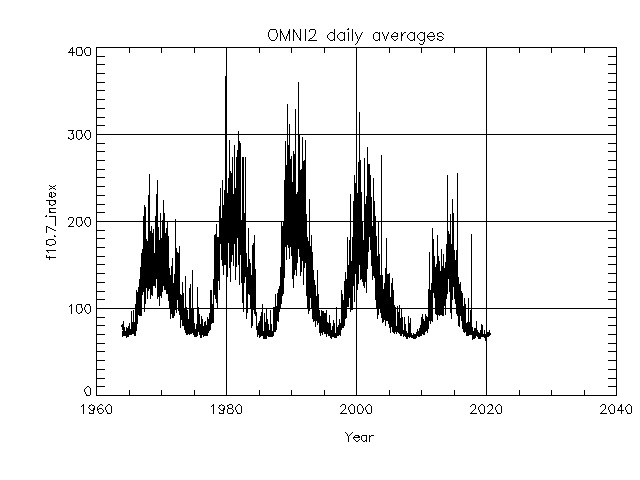
\includegraphics[scale=0.55]{Figuras/jpg_omni2_daily_wSxReptBqw.jpg}
     \end{center}
\end{column}
\end{columns}
\end{frame}

%%%%%%%%%%%%%%%%%%%%%%%%  FRAME  %%%%%%%%%%%%%%%%%%%%%%%%
\begin{frame}
\frametitle{Os Dados - Médias de 27 dias}
\begin{columns}
\begin{column}{0.4\textwidth}
\begin{itemize}
\item Cada ano com 13 ou 14 registros
\item Sinal menos oscilatório em pequenas escalas
\item Tamanho final: $2^{9}$ registros
\end{itemize}
\end{column}
\begin{column}{0.6\textwidth}  %%<--- here
    \begin{center}
     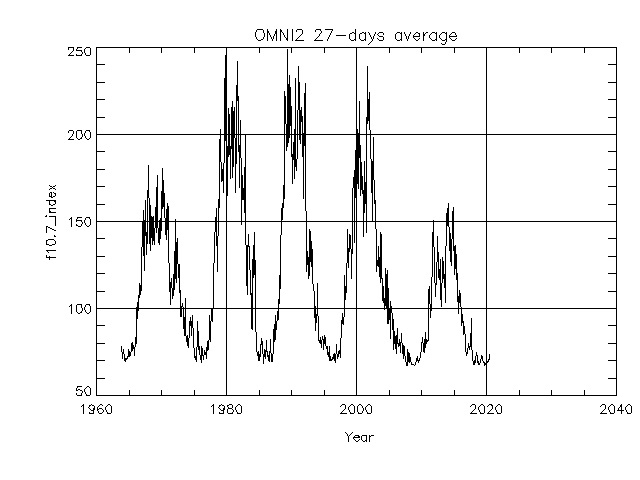
\includegraphics[scale=0.55]{Figuras/jpg_omni2_27day_bdhxX8pSxb.jpg}
     \end{center}
\end{column}
\end{columns}
\end{frame}

%%%%%%%%%%%%%%%%%%%%%%%%  FRAME  %%%%%%%%%%%%%%%%%%%%%%%%
\begin{frame}
\frametitle{Os Dados - Médias anuais}
\begin{columns}
\begin{column}{0.4\textwidth}
\begin{itemize}
\item Dado sem flutuações
\item Característica de longo prazo: variação sinusoidal com período de aprox. onze anos
\item Tamanho final: $2^{5}$ registros
\end{itemize}
\end{column}
\begin{column}{0.6\textwidth}  %%<--- here
    \begin{center}
     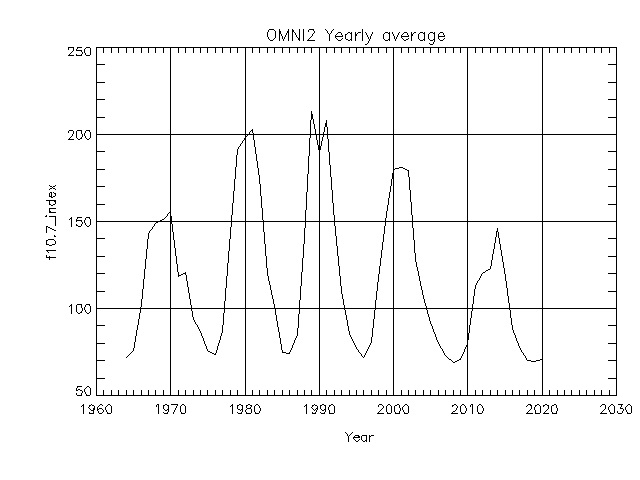
\includegraphics[scale=0.55]{Figuras/jpg_omni2_yearly_3G19RccK_m.jpg}
     \end{center}
\end{column}
\end{columns}
\end{frame}

%%%%%%%%%%%%%%%%%%%%%%%%  FRAME  %%%%%%%%%%%%%%%%%%%%%%%%
\begin{frame}
\frametitle{Os Dados - Exemplo de tratamento}
\begin{center}
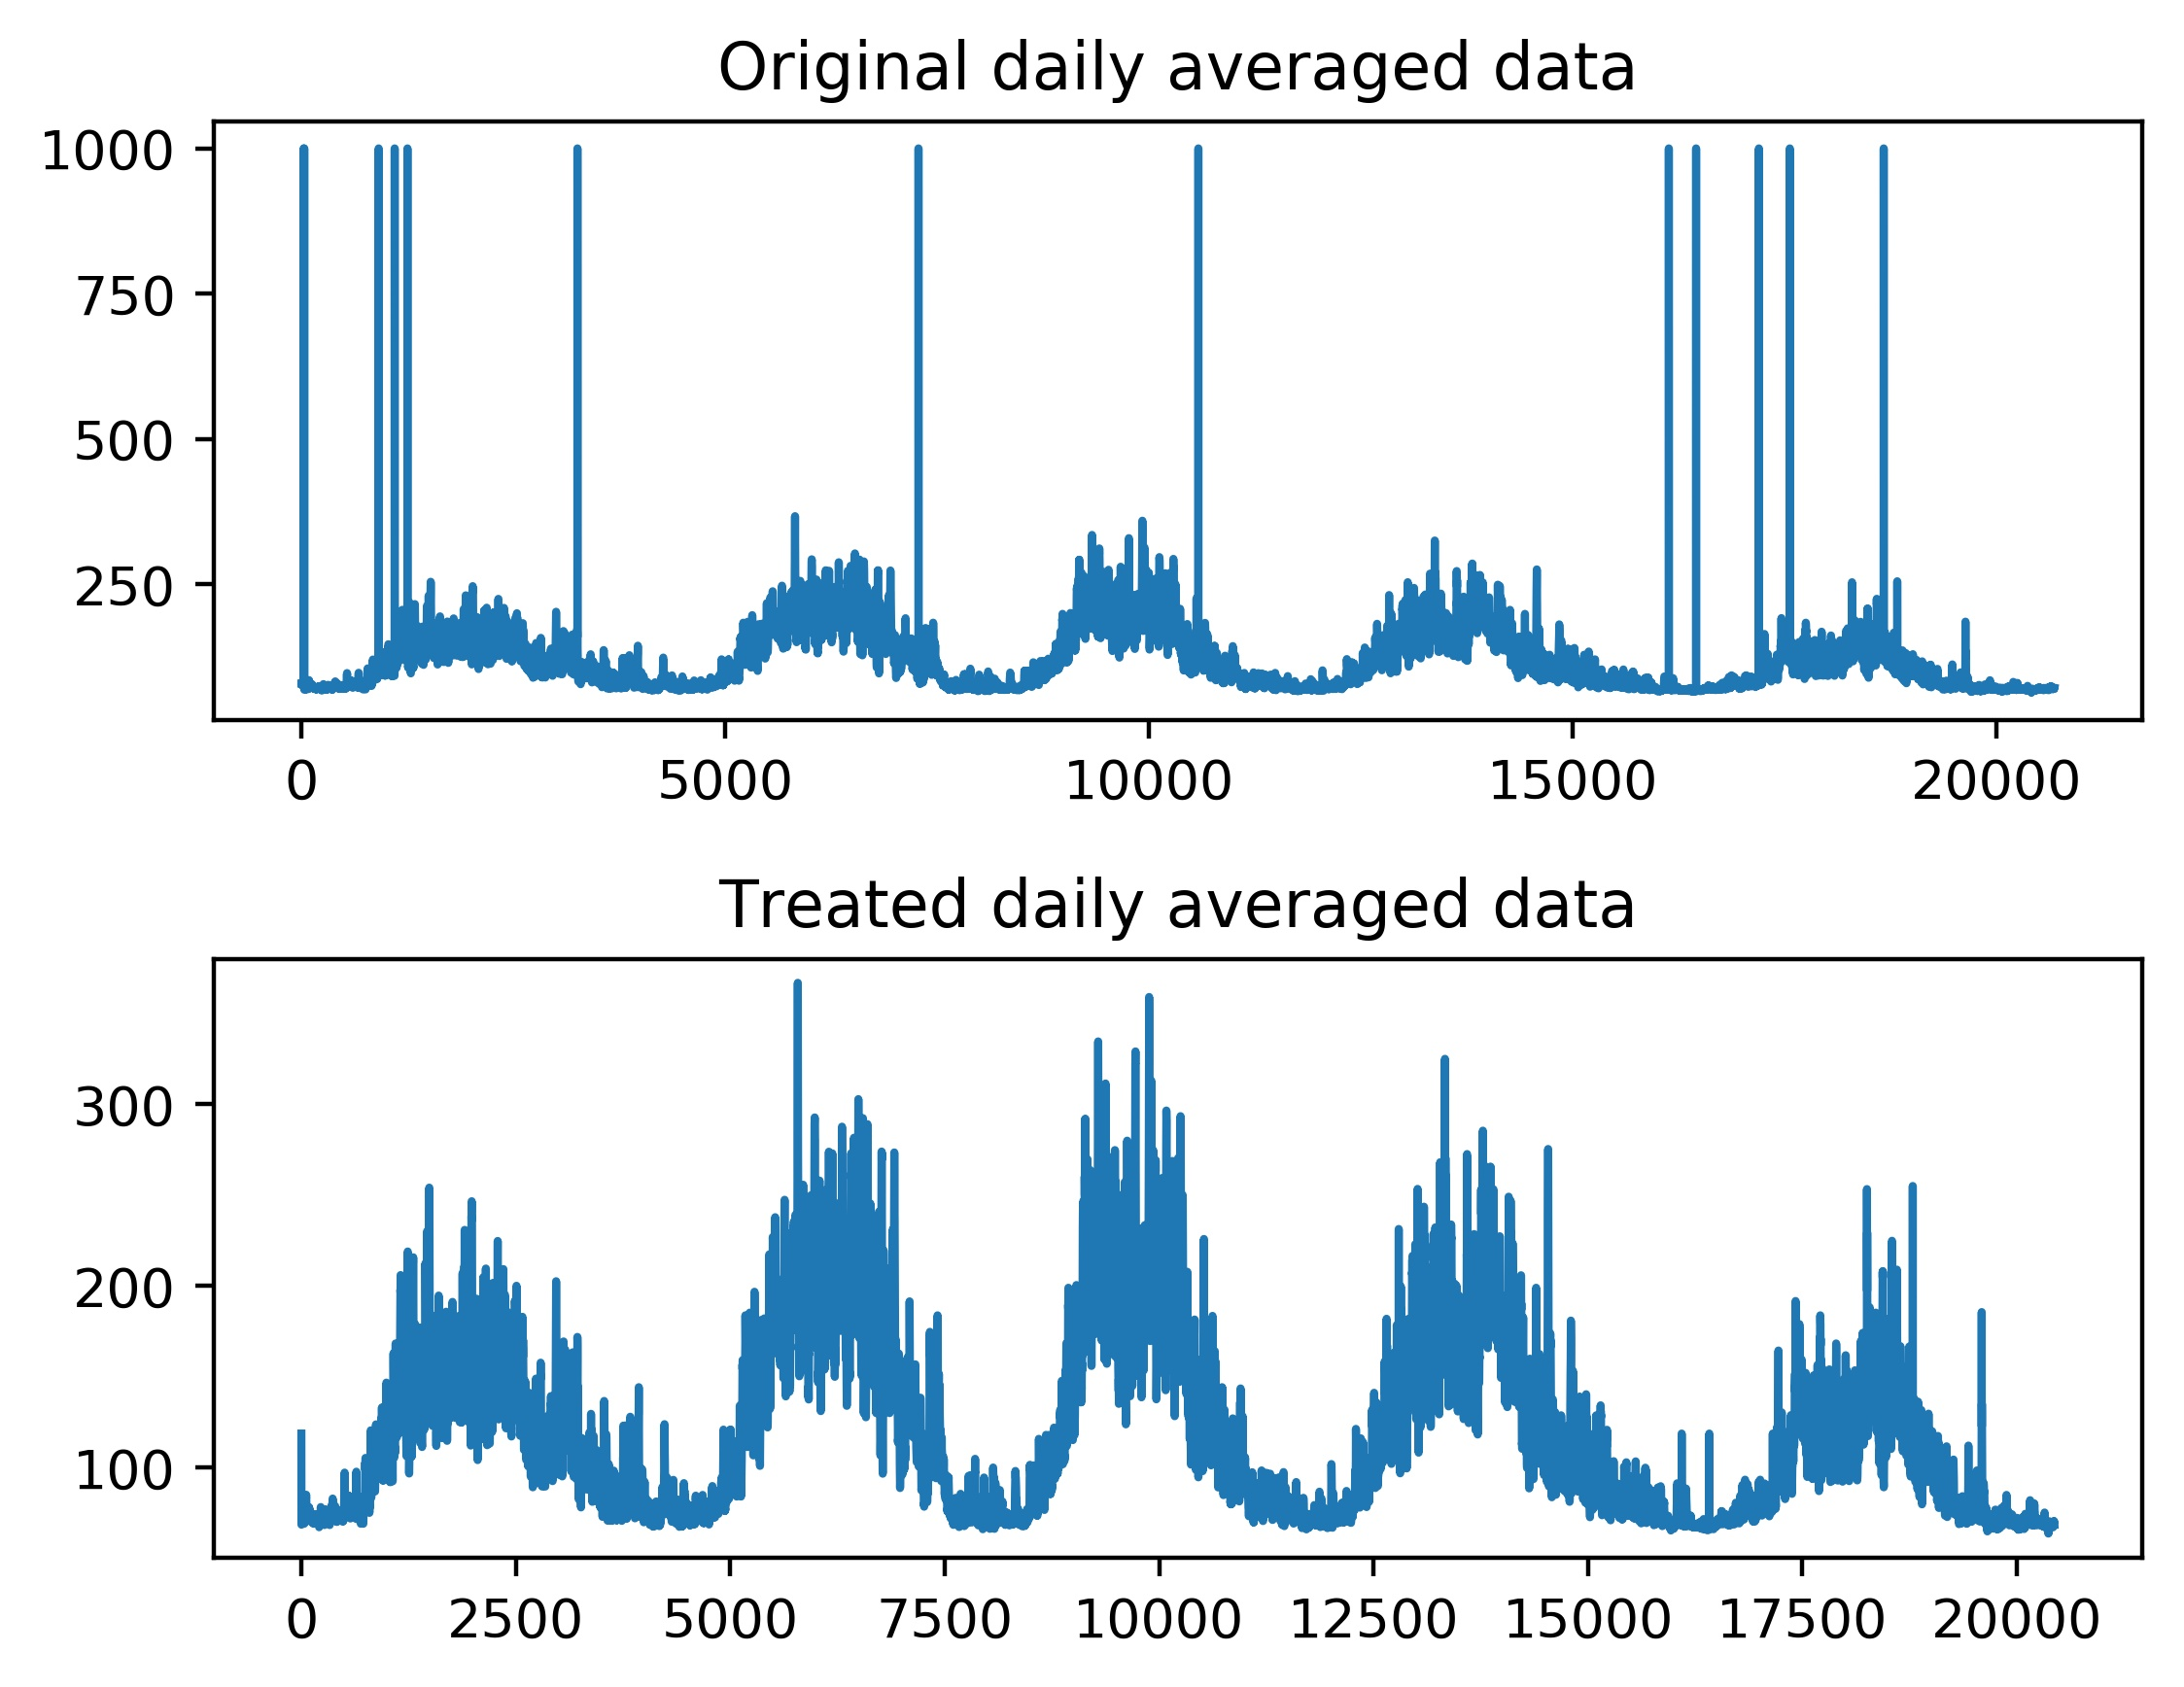
\includegraphics[scale=0.55]{Figuras/final_2.jpg}
\end{center}
\end{frame}

\section{Metodologia de Fourier}

%%%%%%%%%%%%%%%%%%%%%%%%  FRAME  %%%%%%%%%%%%%%%%%%%%%%%%
\begin{frame}
\frametitle{Metodologia de Fourier}
\begin{block}{Análise de Fourier}
Análise de Fourier é uma coleção de técnicas para representar funções (ou sinais) gerais como a combinação linear de funções periódicas. As ferramentas mais úteis na análise de Fourier são suas transformadas.
\end{block}
Transformadas importantes:
\begin{description}
\item[Séries de Fourier] 
\item[Transformada Contínua de Fourier] 
\item[Transformada Discreta de Fourier] 
\end{description}
\end{frame}

%%%%%%%%%%%%%%%%%%%%%%%%  FRAME  %%%%%%%%%%%%%%%%%%%%%%%%
\begin{frame}
\frametitle{Séries de Fourier}
\begin{itemize}
\item Representa funções como uma soma infinita de senos e cossenos: 
\begin{equation*}
f(x) = \frac{a_{0}}{2}+\sum_{k=1}^{\infty}a_{k} \cos kx + \sum_{k=1}^{\infty}b_{k} \sin kx,  \quad x \in [-\pi, \pi]
\end{equation*}
\item $a_{k}$ e $b_{k}$ são os coeficientes de Fourier
\item Os senos e cossenos são as bases % ou os modos
\item $k$ é o número de onda, ou a quantidade de ciclos dentro do intervalo $[-\pi, \pi]$
\end{itemize}
\end{frame}

%%%%%%%%%%%%%%%%%%%%%%%%  FRAME  %%%%%%%%%%%%%%%%%%%%%%%%
\begin{frame}
\frametitle{Séries de Fourier}
\begin{center}
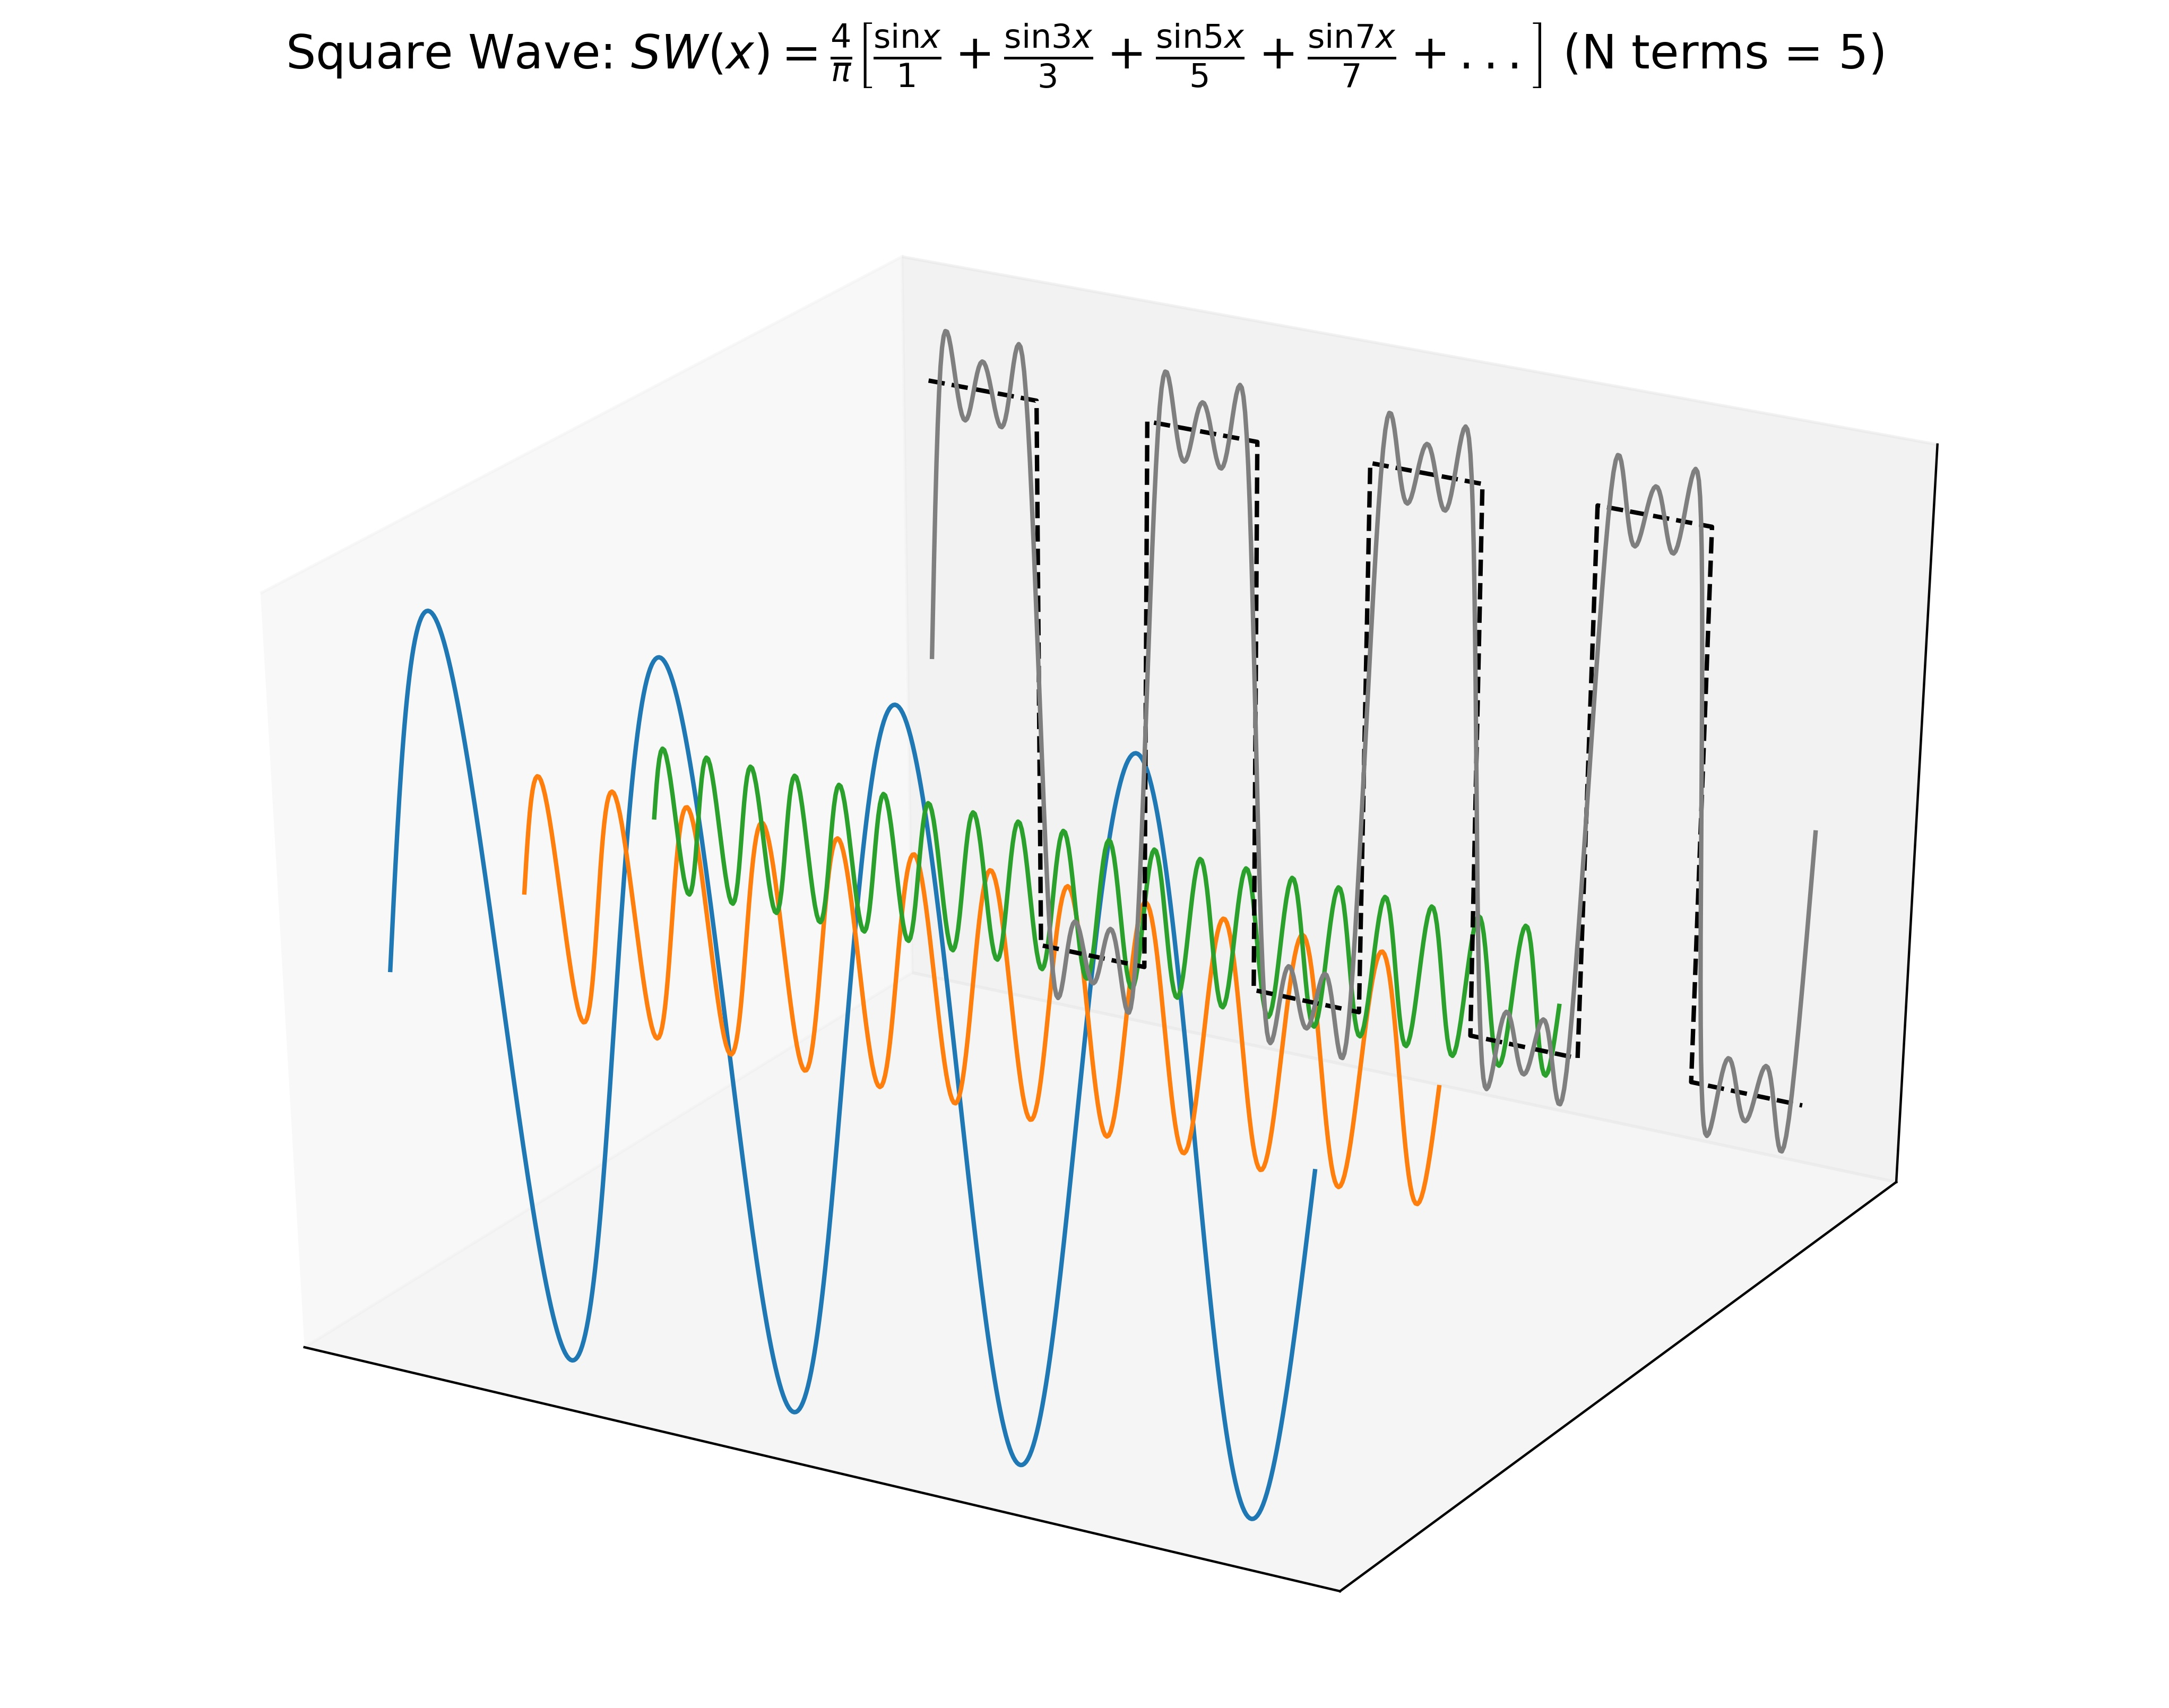
\includegraphics[scale=0.4]{Figuras/sqw5.jpg}
\end{center}
\end{frame}
\begin{frame}
\frametitle{Séries de Fourier}
\begin{center}
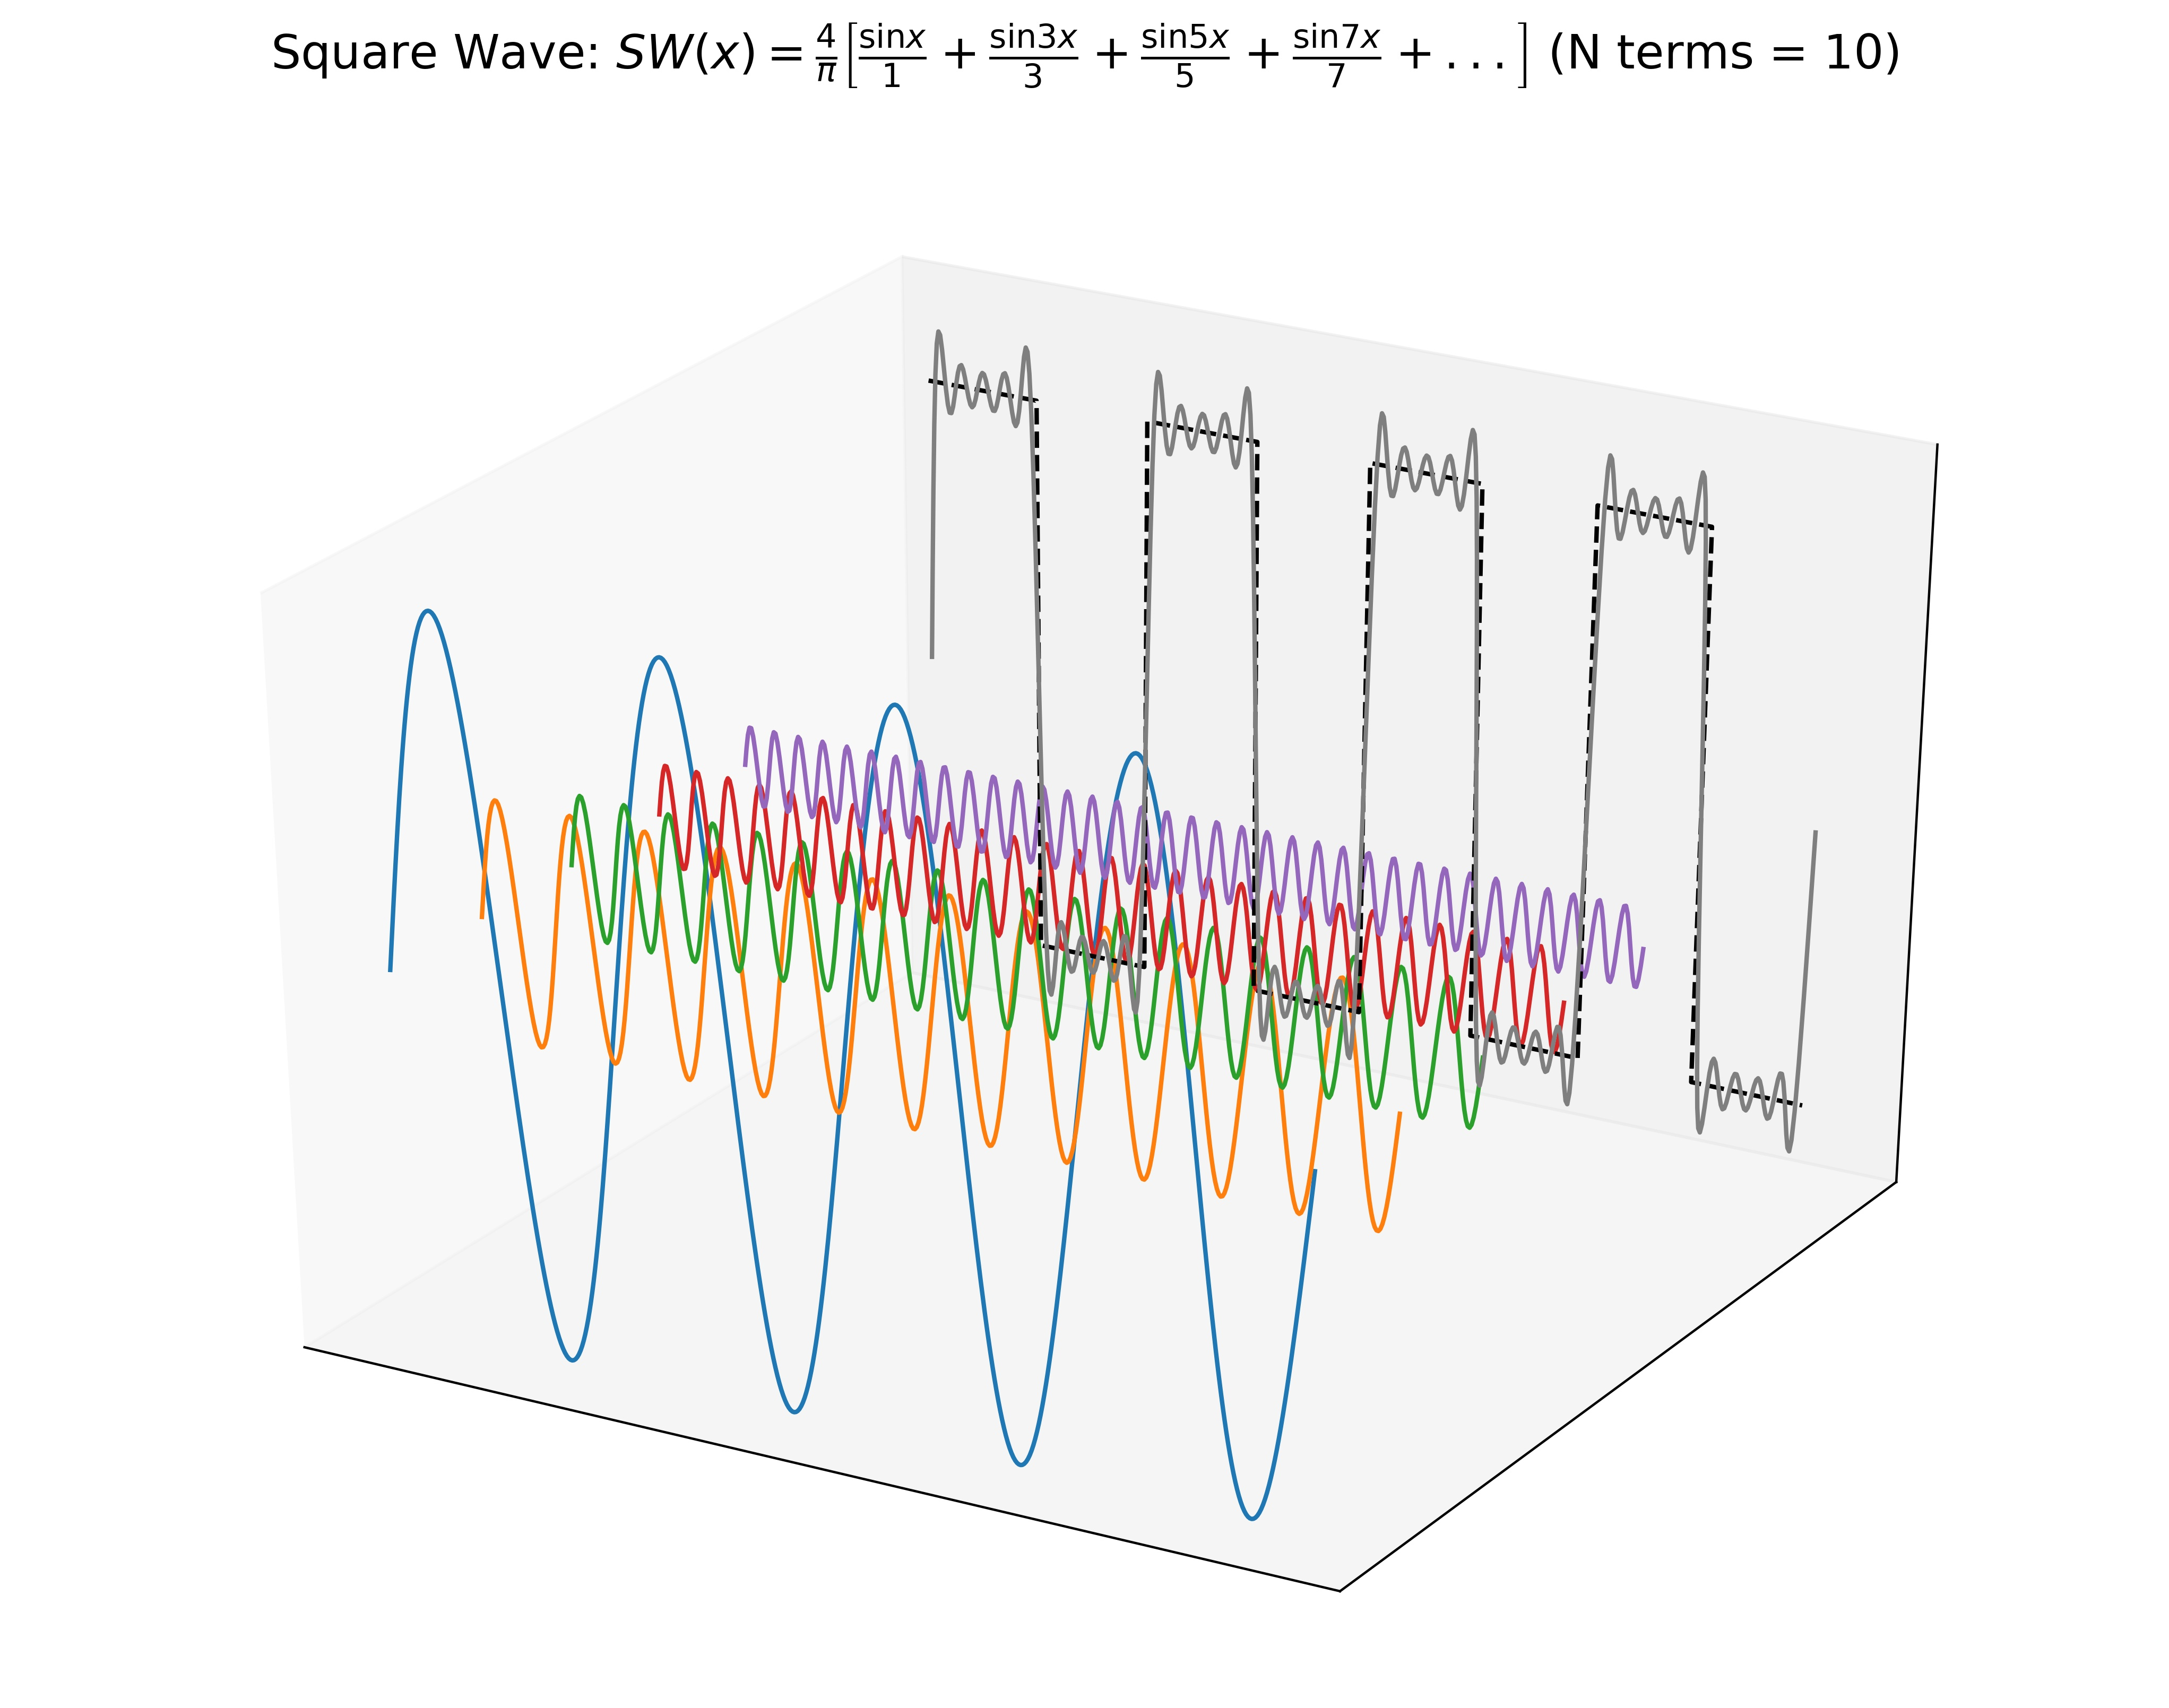
\includegraphics[scale=0.4]{Figuras/sqw10.jpg}
\end{center}
\end{frame}
\begin{frame}
\frametitle{Séries de Fourier}
\begin{center}
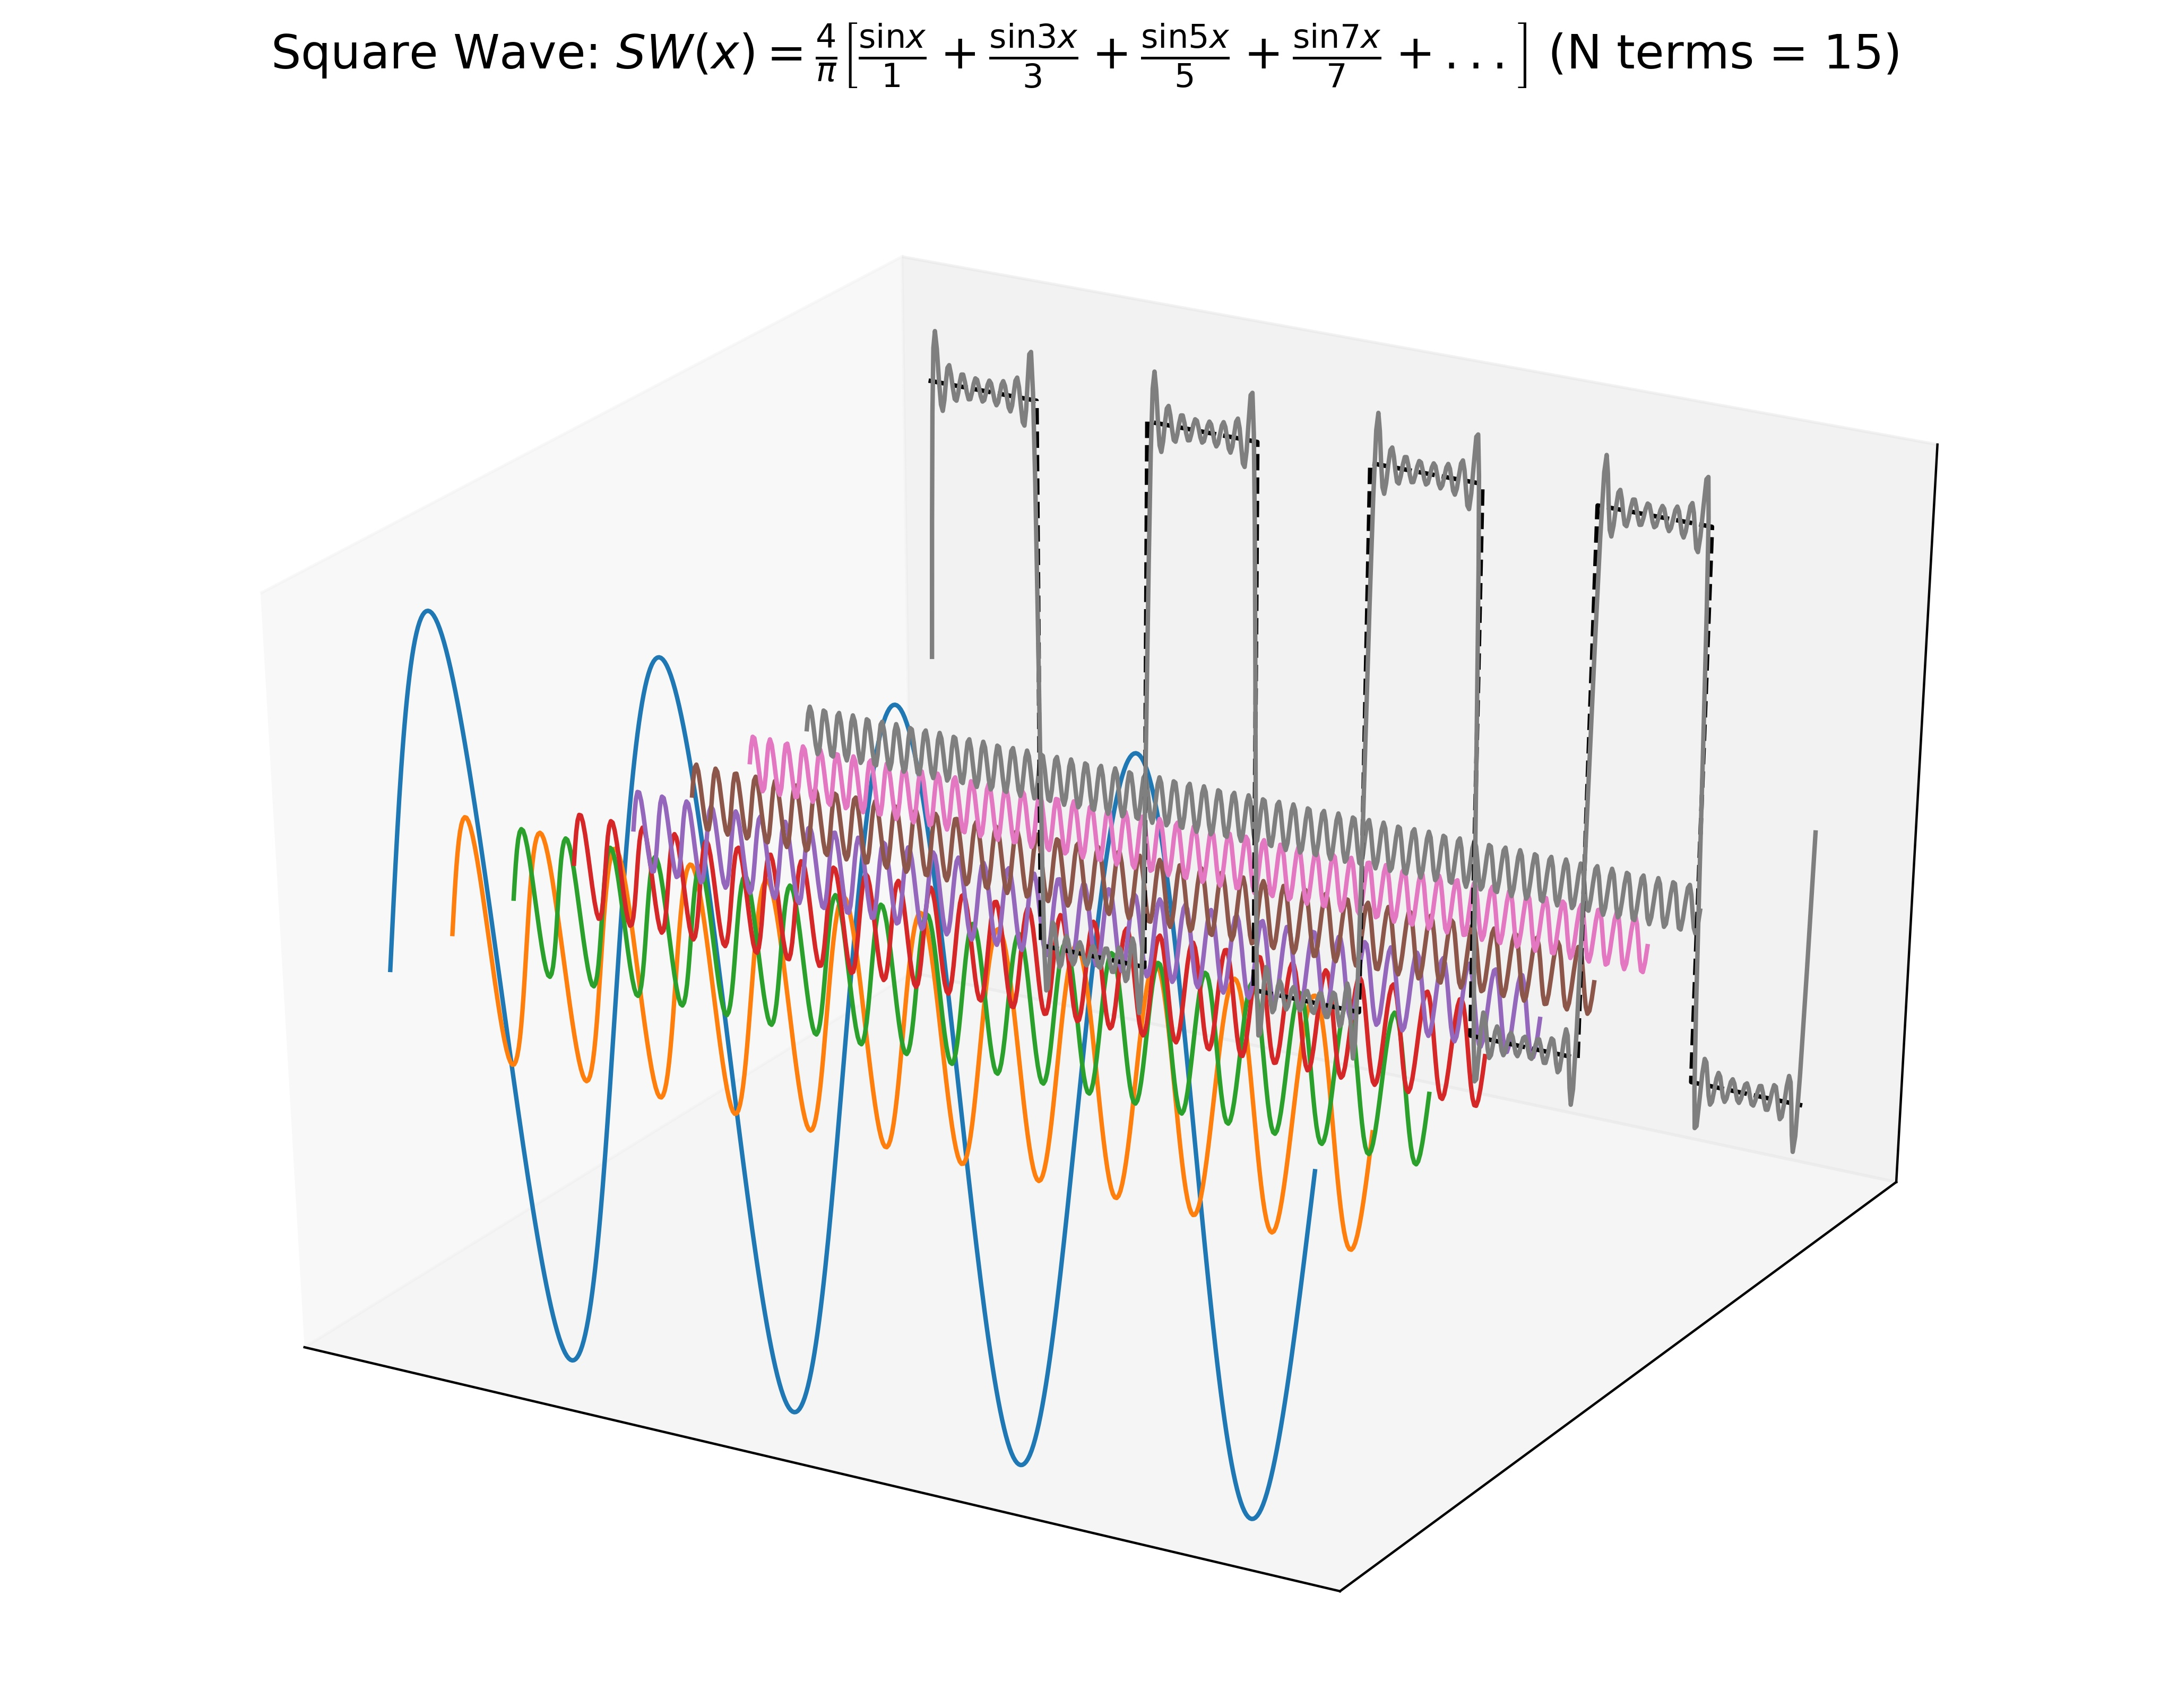
\includegraphics[scale=0.4]{Figuras/sqw15.jpg}
\end{center}
\end{frame}
\begin{frame}
\frametitle{Séries de Fourier}
\begin{center}
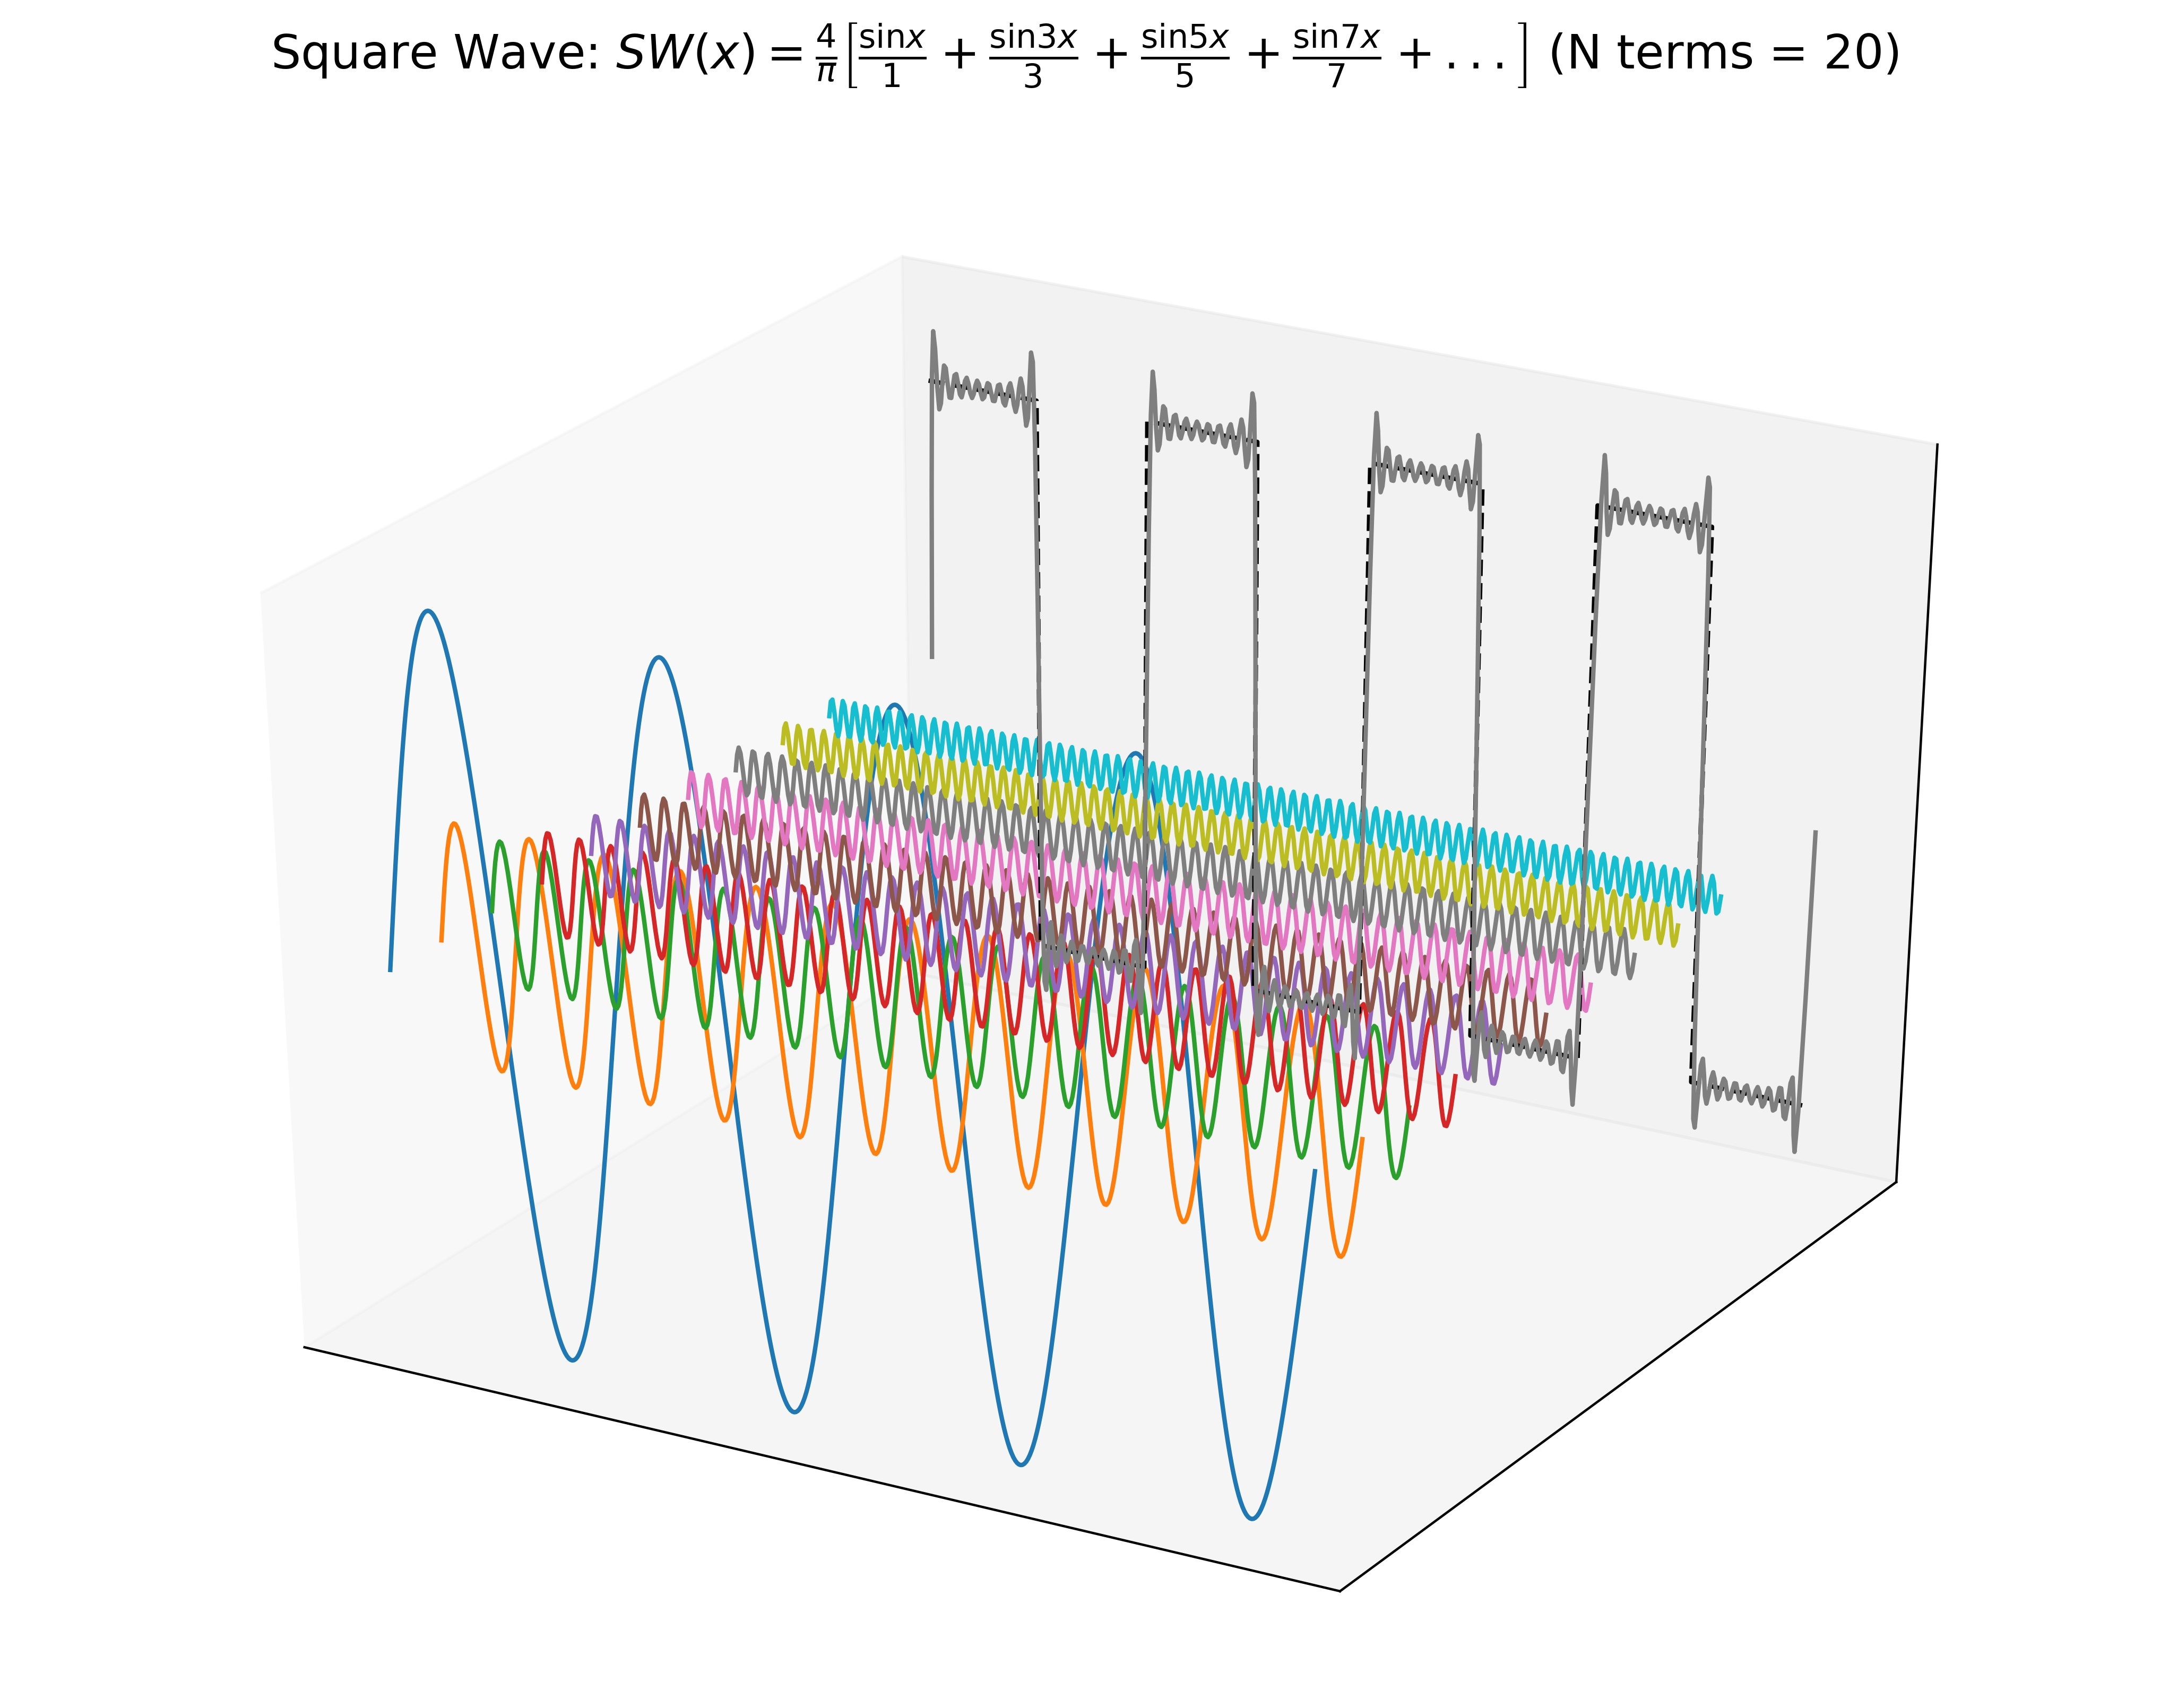
\includegraphics[scale=0.4]{Figuras/sqw20.jpg}
\end{center}
\end{frame}

%%%%%%%%%%%%%%%%%%%%%%%%  FRAME  %%%%%%%%%%%%%%%%%%%%%%%%
\begin{frame}
\frametitle{Séries de Fourier}
\begin{center}
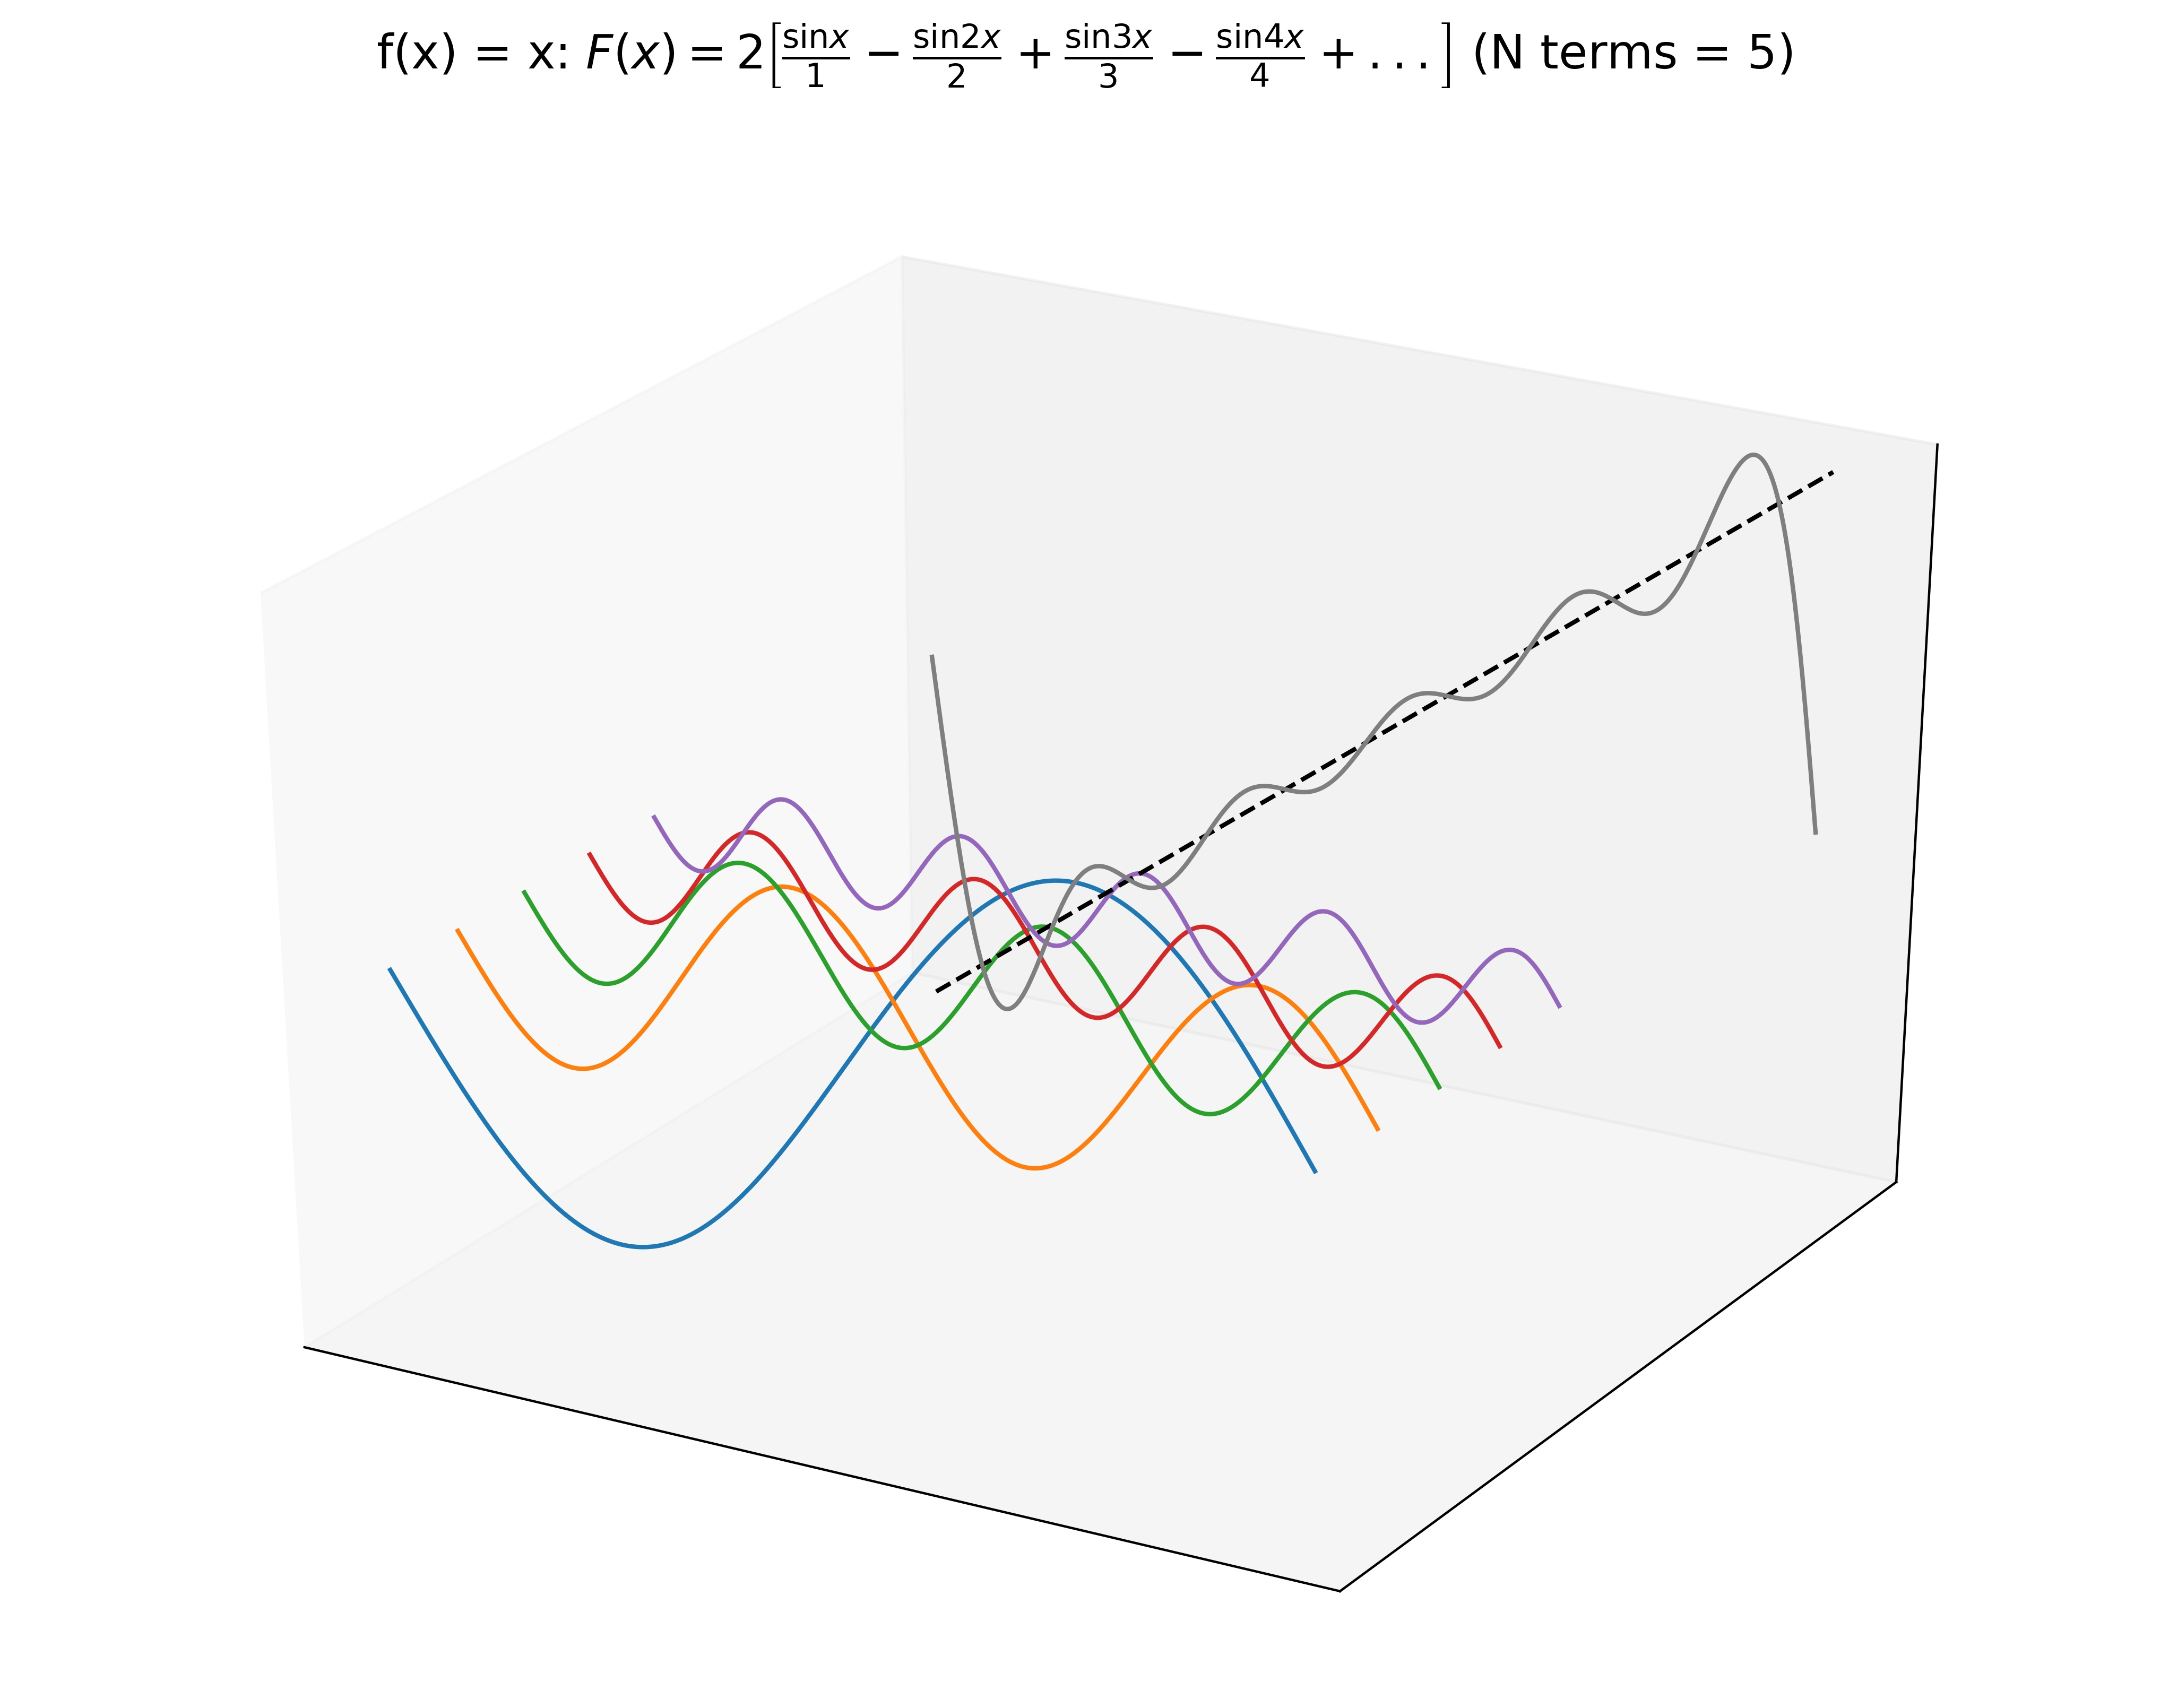
\includegraphics[scale=0.4]{Figuras/x5.jpg}
\end{center}
\end{frame}
\begin{frame}
\frametitle{Séries de Fourier}
\begin{center}
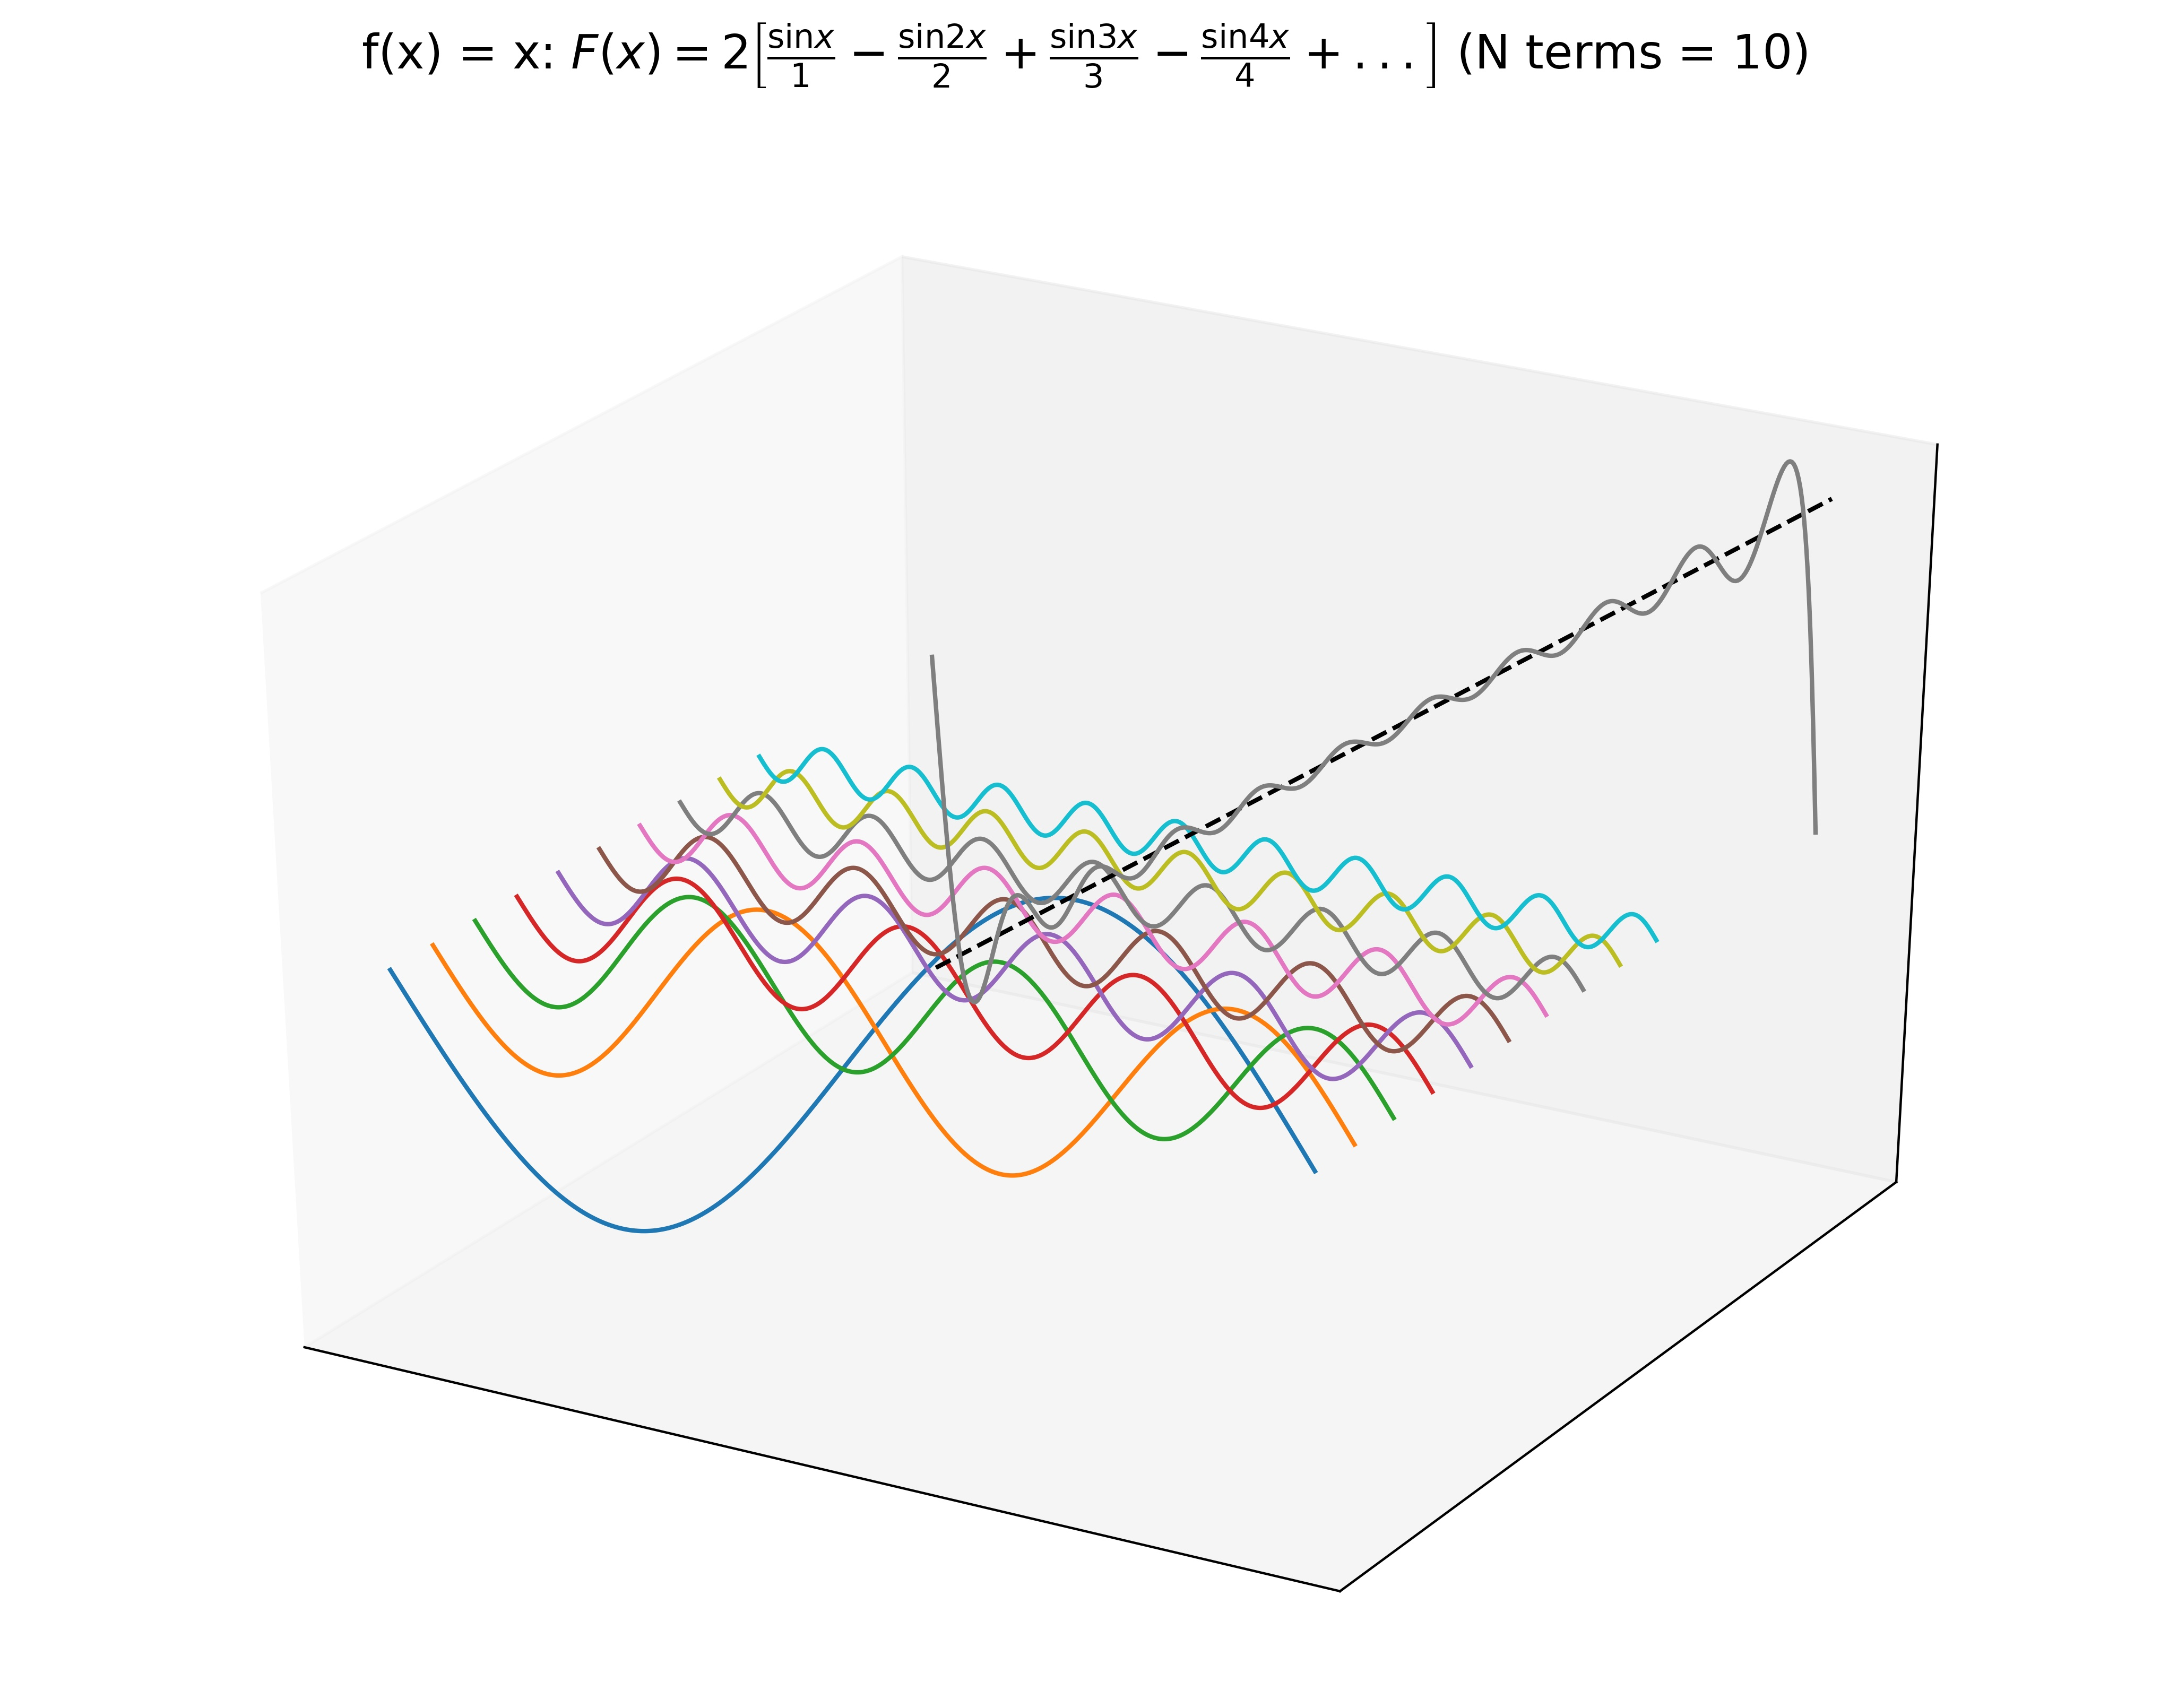
\includegraphics[scale=0.4]{Figuras/x10.jpg}
\end{center}
\end{frame}
\begin{frame}
\frametitle{Séries de Fourier}
\begin{center}
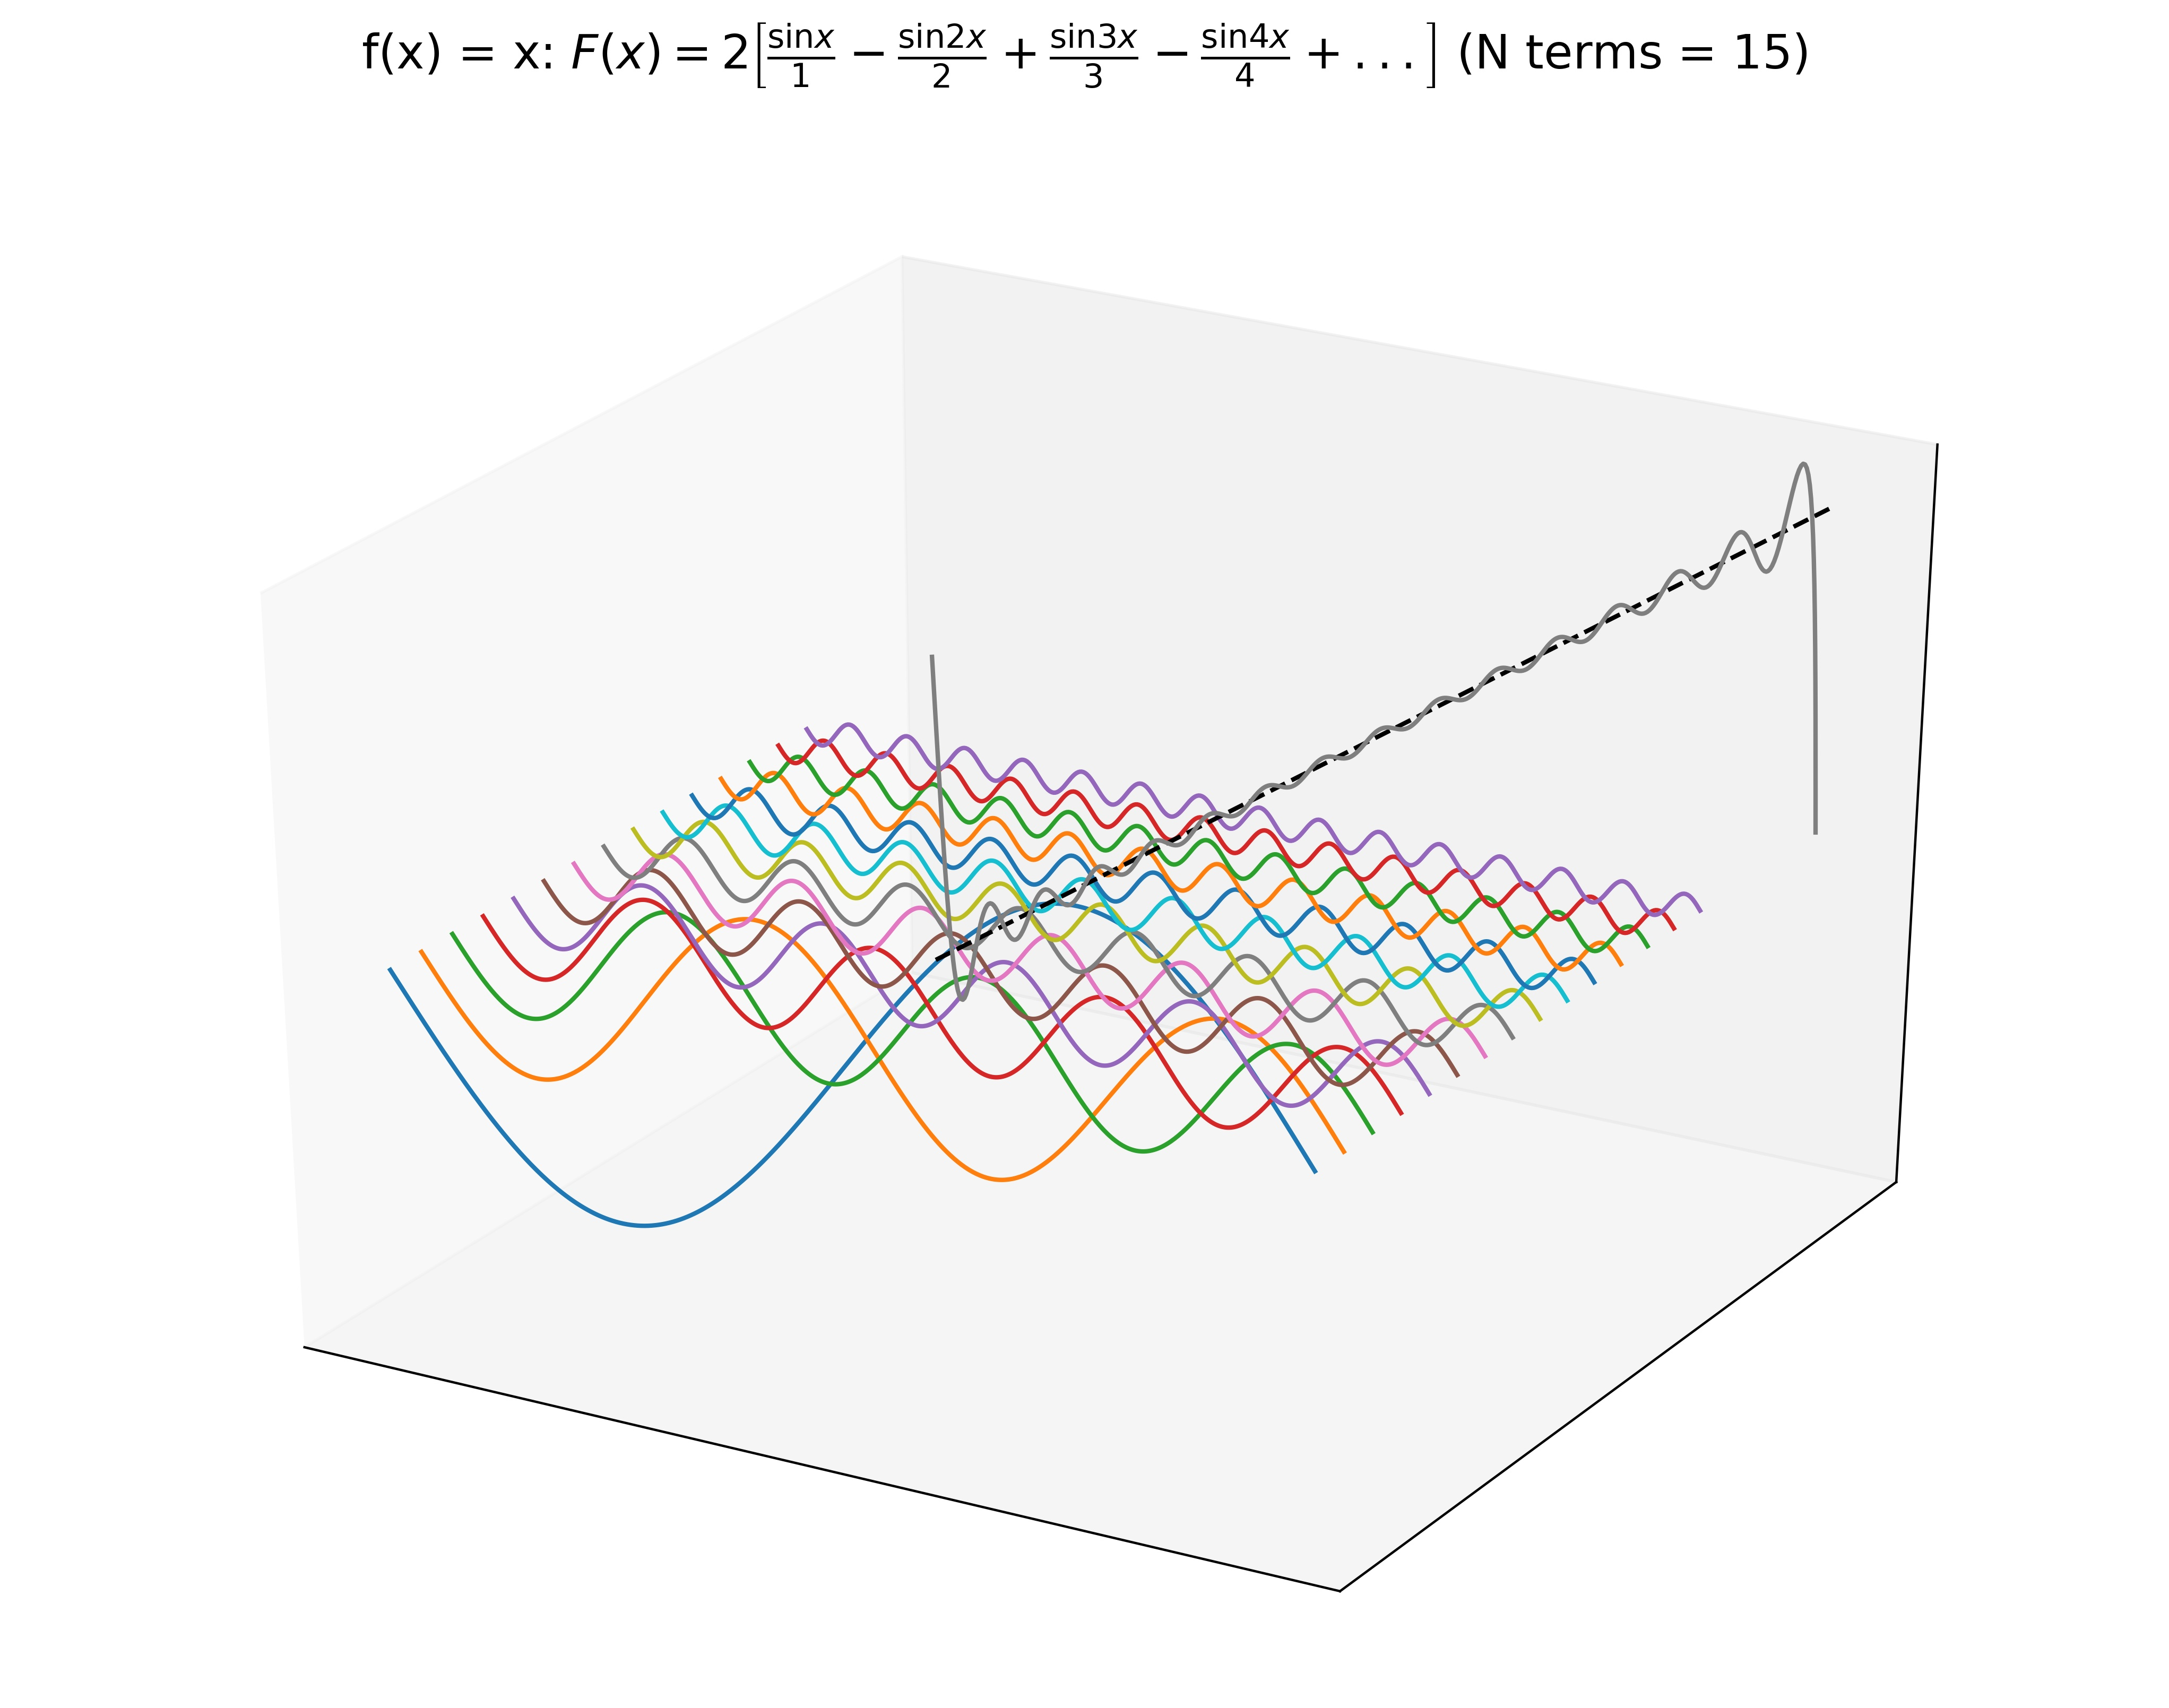
\includegraphics[scale=0.4]{Figuras/x15.jpg}
\end{center}
\end{frame}
\begin{frame}
\frametitle{Séries de Fourier}
\begin{center}
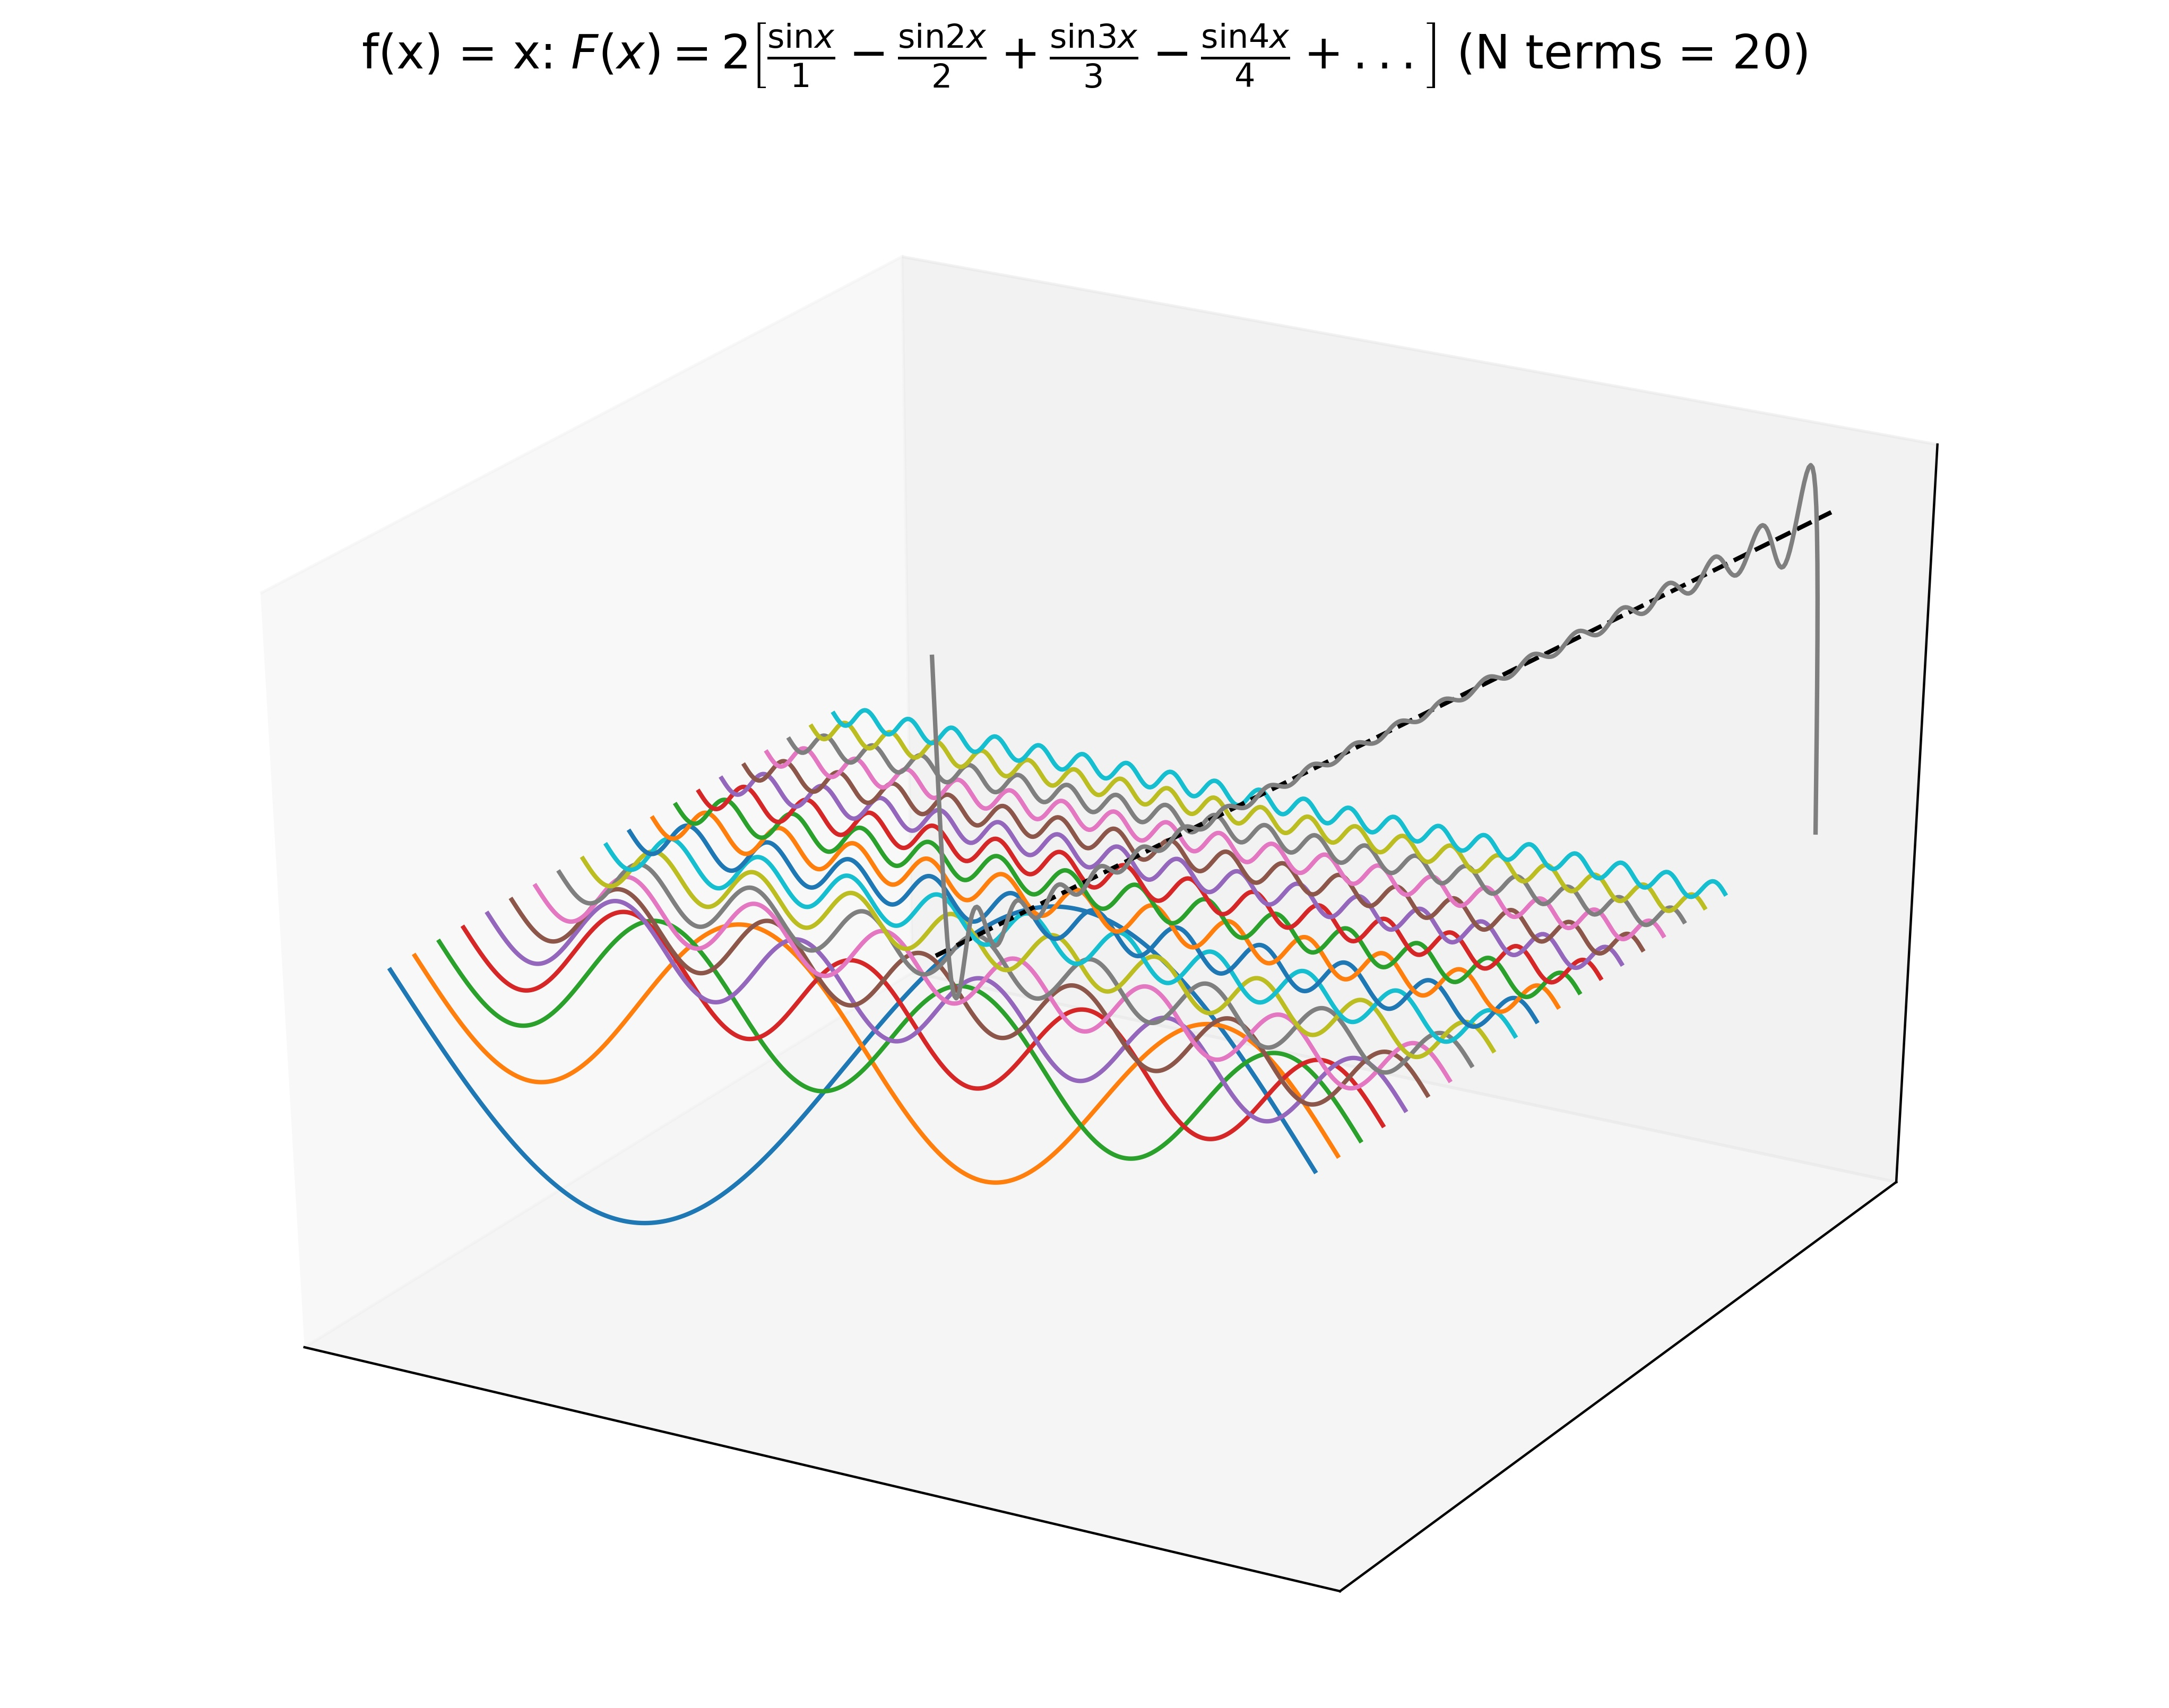
\includegraphics[scale=0.4]{Figuras/x20.jpg}
\end{center}
\end{frame}

%%%%%%%%%%%%%%%%%%%%%%%%  FRAME  %%%%%%%%%%%%%%%%%%%%%%%%
\begin{frame}
\frametitle{Transformada Contínua de Fourier}
\begin{itemize}
\item Transforma uma função definida no domínio do tempo para o domínio da frequência
\item Transformada direta:
\begin{equation*}
F(\omega)=\int_{-\infty}^{\infty}f(t)\exp^{-i\omega t}dt
\end{equation*}
\item Transformada inversa:
\begin{equation*}
f(t)=\int_{-\infty}^{\infty}F(\omega)\exp^{i\omega t}d\omega
\end{equation*}
\item $\omega = 2\pi/T$ é a frequência em radianos por unidade de tempo
\end{itemize}
\end{frame}

%%%%%%%%%%%%%%%%%%%%%%%%  FRAME  %%%%%%%%%%%%%%%%%%%%%%%%
\begin{frame}
\frametitle{Espectro de Potência}
%\end{block}
\begin{itemize}
\item É o quadrado da Transformada de Fourier, representando a energia associada a cada componente de frequência do sinal
\begin{equation*}
F(\omega)F^{*}(\omega)=|F(\omega)|^{2} 
\end{equation*}
\item Em outras palavras, é o quadrado dos coeficientes, $a_{k}^{2} + b_{k}^{2}$, em função da frequência
\end{itemize}
\end{frame}
%
\begin{frame}
\frametitle{Espectro de Potência}
\begin{center}
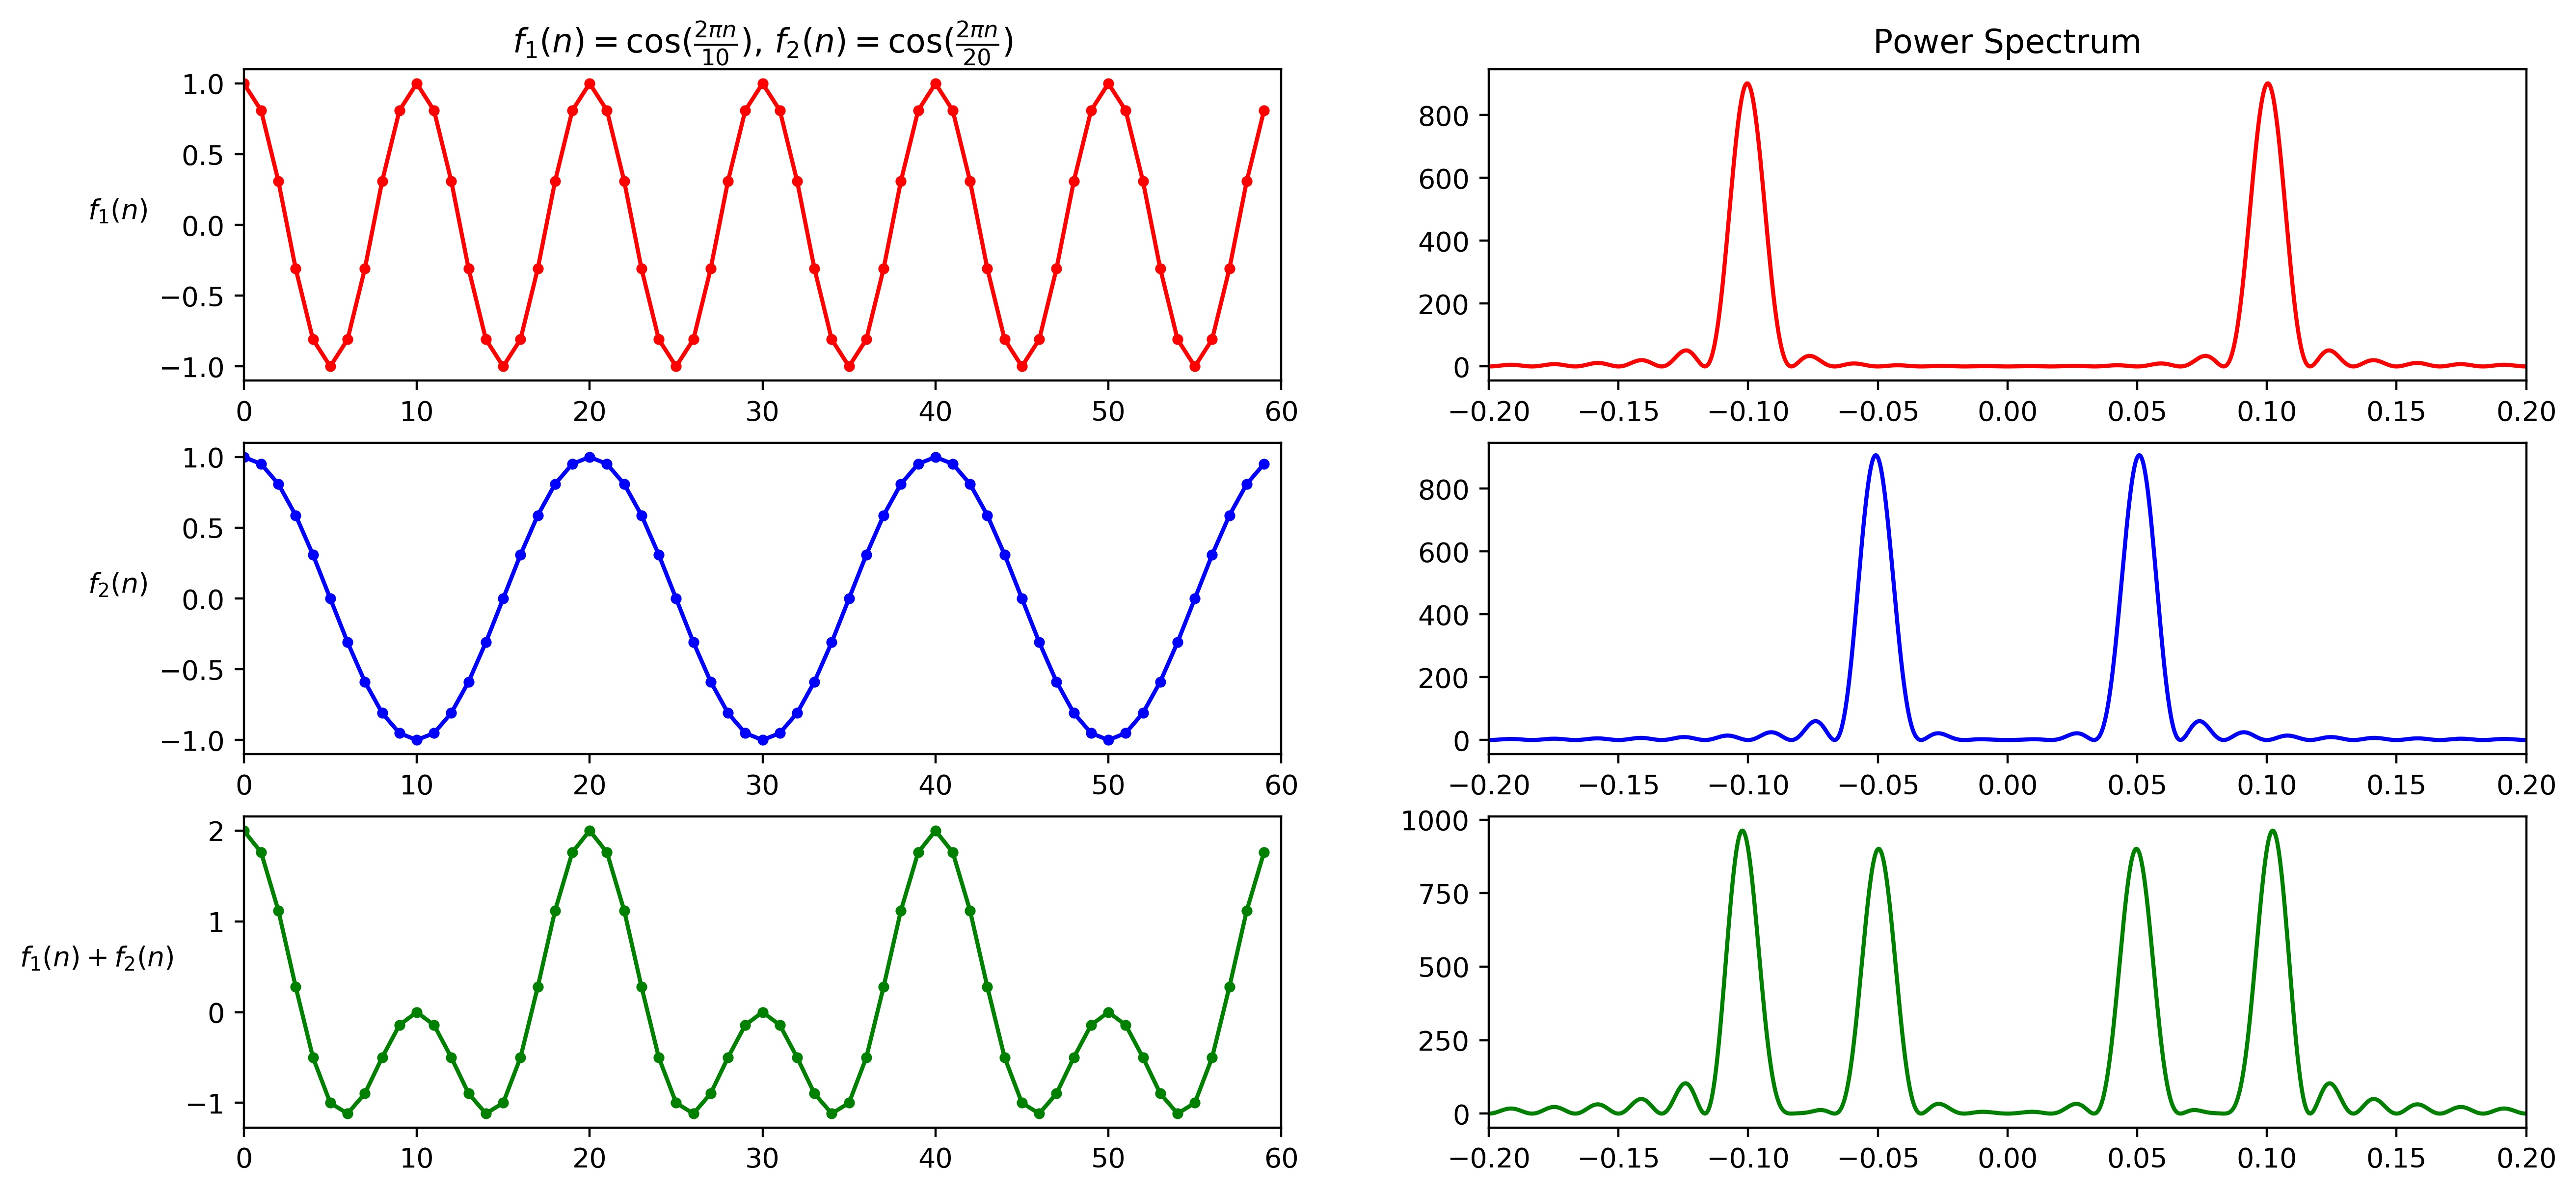
\includegraphics[scale=0.37]{Figuras/ft_exemplo.jpg}
\end{center}
\end{frame}

%%%%%%%%%%%%%%%%%%%%%%%%  FRAME  %%%%%%%%%%%%%%%%%%%%%%%%
\begin{frame}[fragile]
\frametitle{Transformada Discreta de Fourier - Algoritmo FFT}
\begin{itemize}
\item Contrapartida discreta da Transformada Contínua de Fourier
\item Esta transformada se aplica a uma sequência finita de registros (tomadas num intervalo uniforme de tempo), convertendo-a numa sequência de mesmo tamanho em função da frequência
\item Implementação numérica: FFT (Fast Fourier Transform)
% Por lidar com dados finitos
\item Em \texttt{Python} (com o pacote \texttt{Numpy}):
\begin{lstlisting}[language=python,style=mystyle2]
import numpy.fft as fft
dado = np.genfromtxt('data.txt') # importando dado
dado_ft = fft.fft(dado) # transf. discreta de Fourier
dado_ps = abs(dado_ft)**2 # espectro de potencia 
\end{lstlisting}
\end{itemize}
\end{frame}

%%%%%%%%%%%%%%%%%%%%%%%%  FRAME  %%%%%%%%%%%%%%%%%%%%%%%%
%\begin{frame}
%%\label{pictures}
%\frametitle{Pictures}
%\begin{figure}
%\includegraphics[scale=0.5]{lion}
%\caption{lion!!}
%\end{figure}
%Excepteur sint occaecat cupidatat non proident, sunt in culpa qui officia deserunt mollit anim id est laborum.
%\end{frame}

\section{Resultados e Discussão}

%%%%%%%%%%%%%%%%%%%%%%%%  FRAME  %%%%%%%%%%%%%%%%%%%%%%%%
\begin{frame}
\frametitle{Resultados - Espectro de potência vs frequência}
\begin{center}
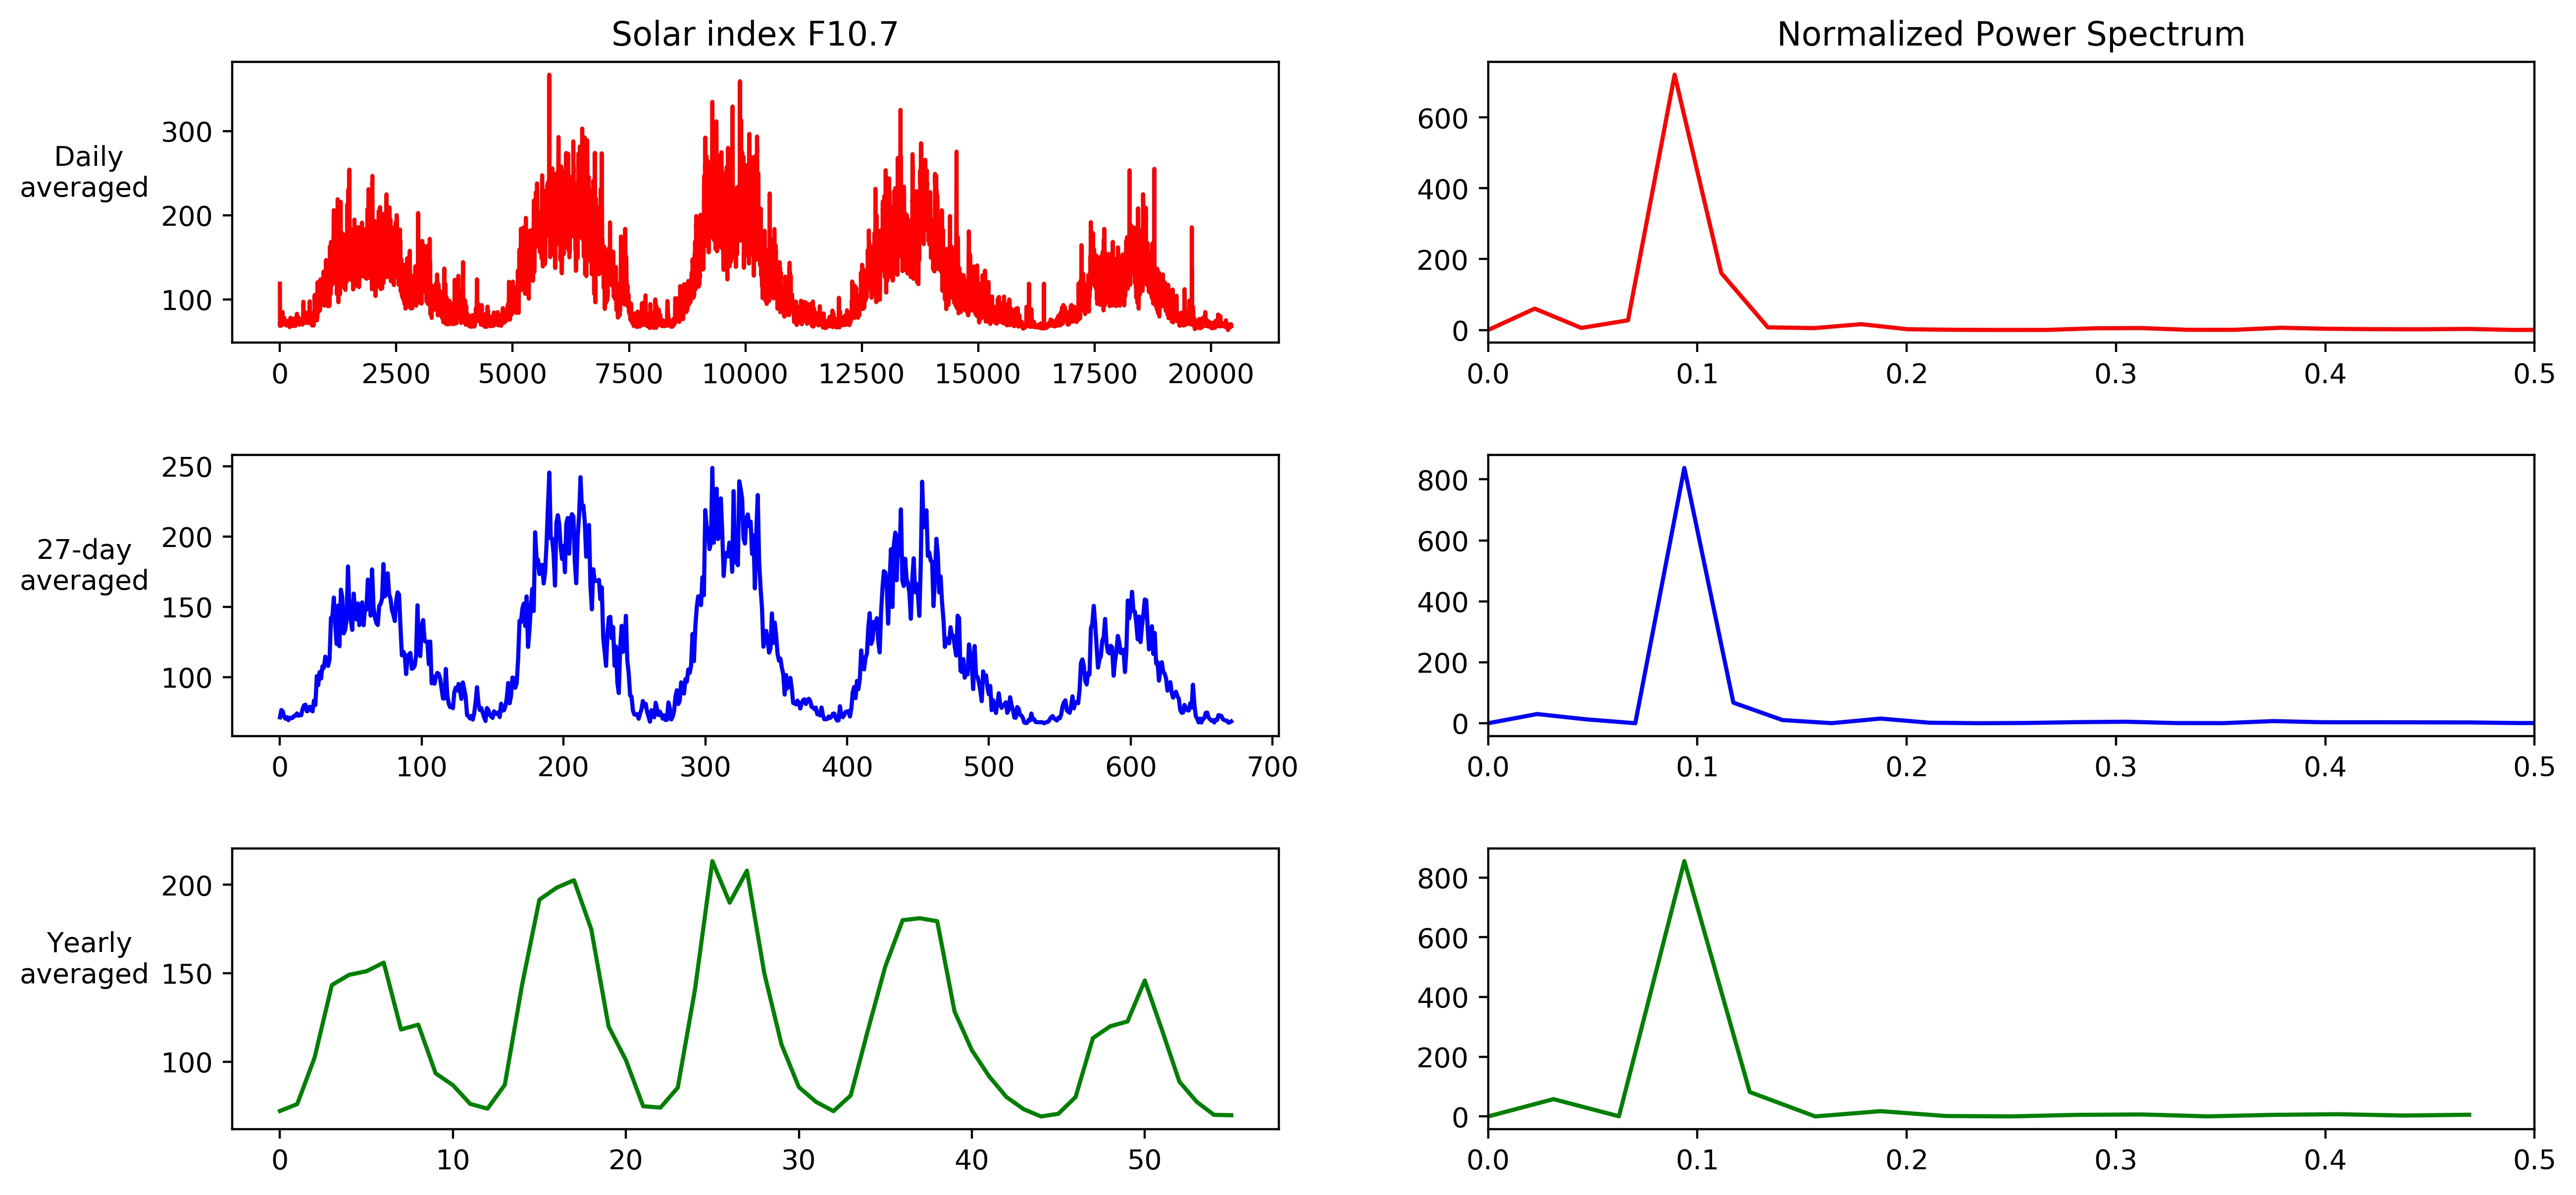
\includegraphics[scale=0.376]{Figuras/final_f.jpg}
\end{center}
\small
Somente metade dos coeficientes são exibidos, visto que o output é simétrico. O resultado indica que o pico da atividade solar ocorre em frequências baixas (em ciclos mais longos que um ano).
\end{frame}

%%%%%%%%%%%%%%%%%%%%%%%%  FRAME  %%%%%%%%%%%%%%%%%%%%%%%%
\begin{frame}
\frametitle{Resultados - Espectro de potência vs tempo}
\begin{center}
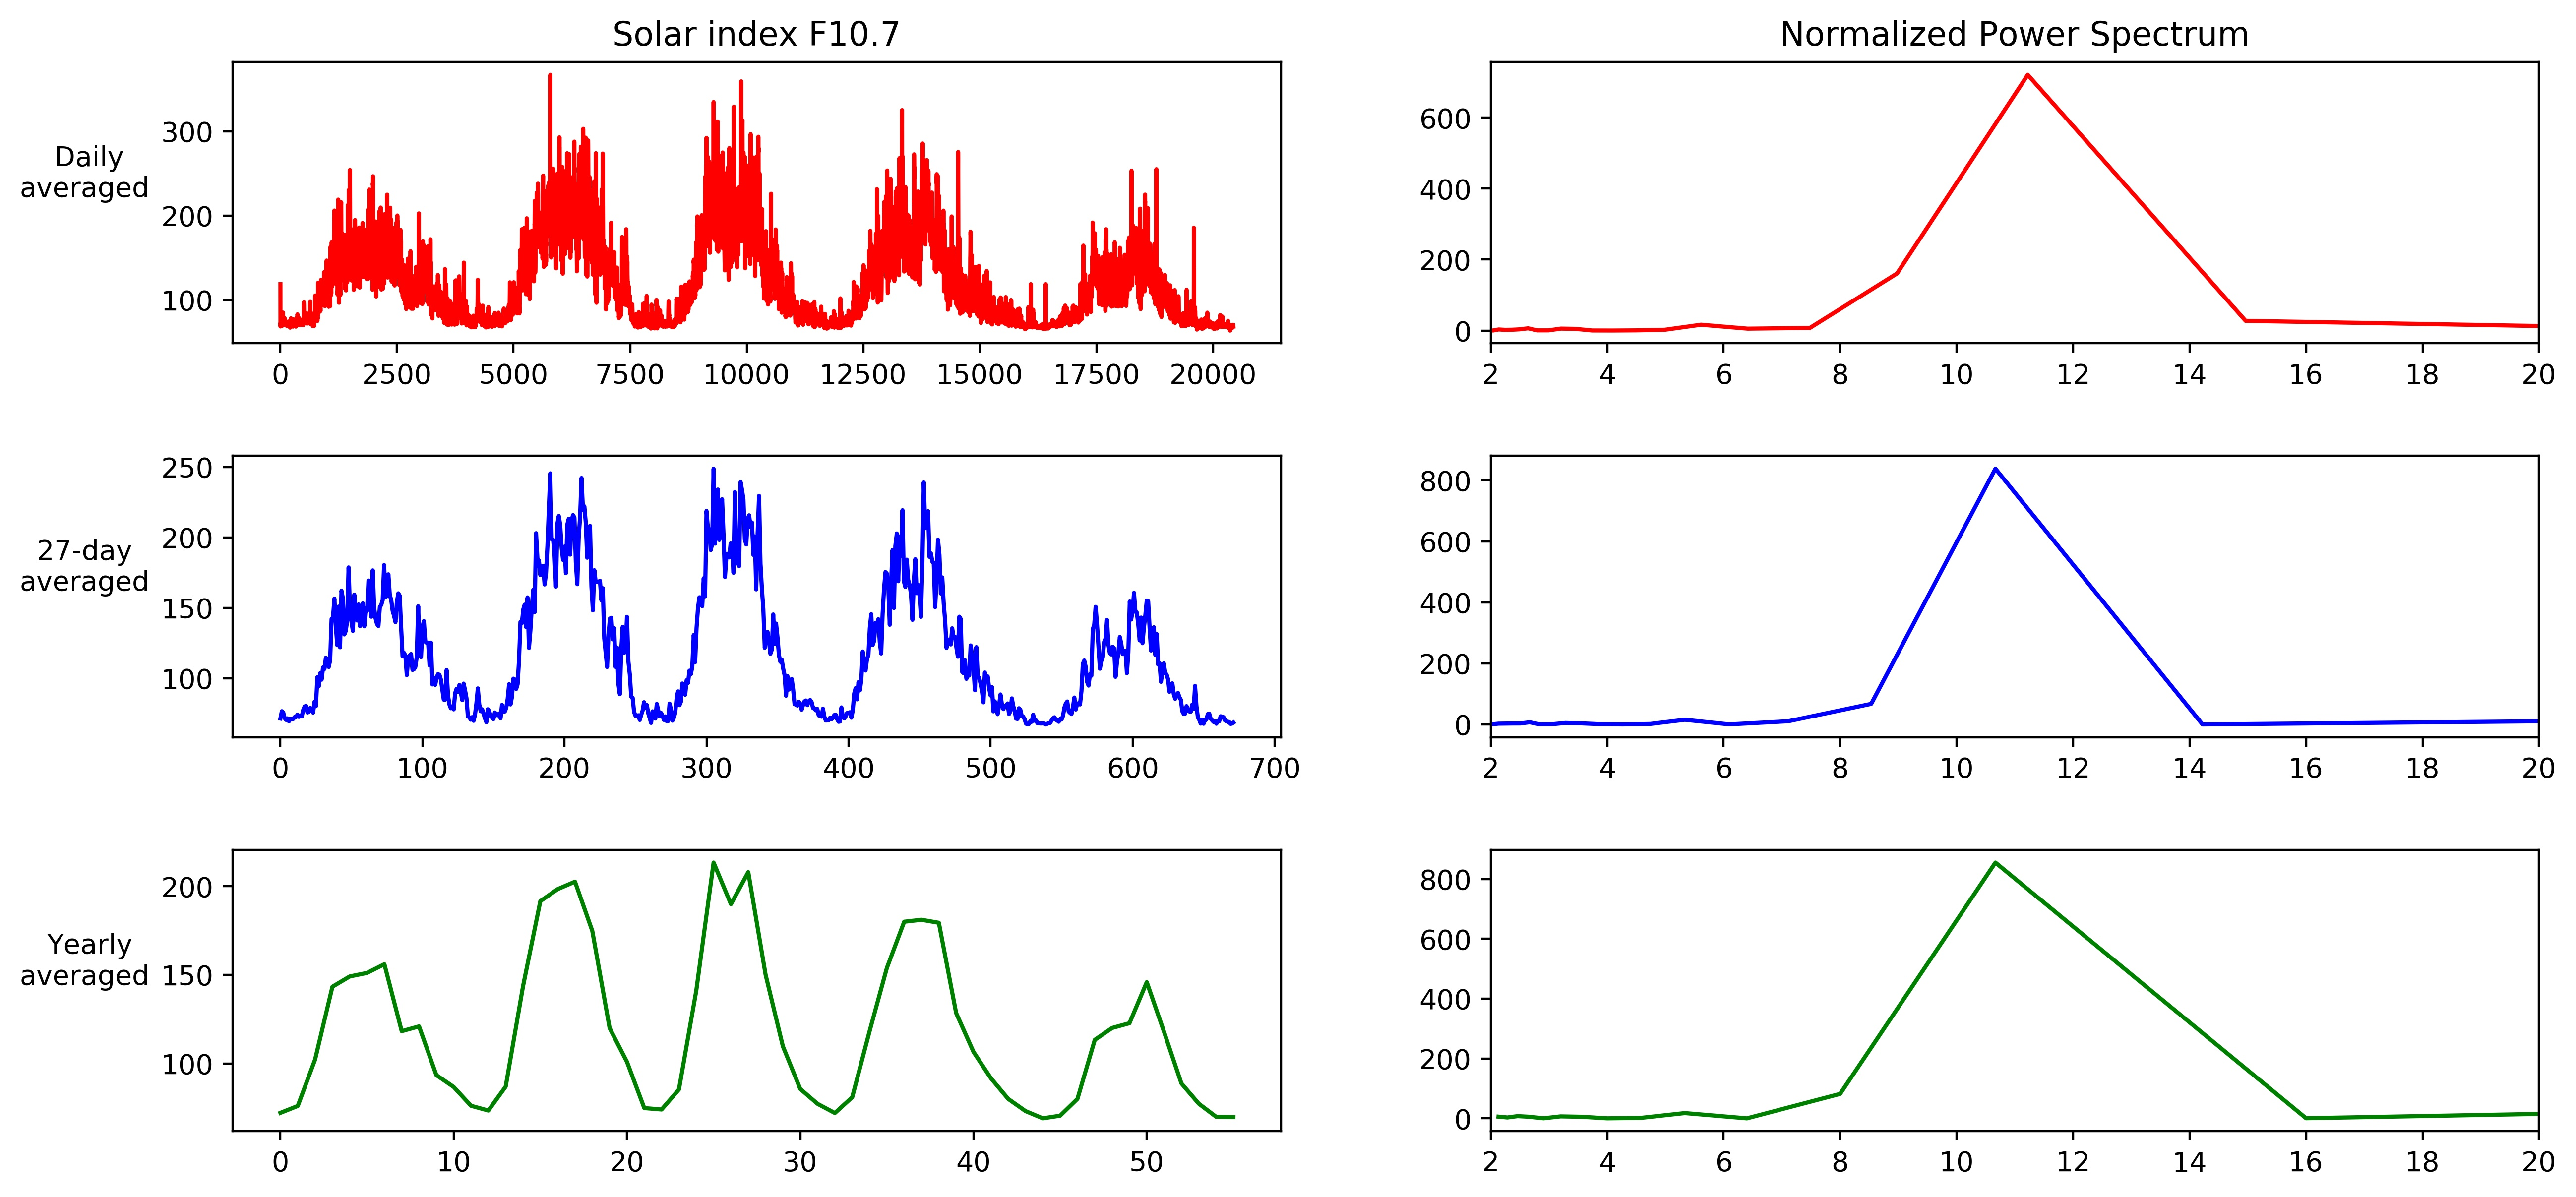
\includegraphics[scale=0.376]{Figuras/final_t2.jpg}
\end{center}
Espectro de potência em função do tempo. O pico de atividade solar ocorre aproximadamente a cada onze anos.
\end{frame}

%%%%%%%%%%%%%%%%%%%%%%%%  FRAME  %%%%%%%%%%%%%%%%%%%%%%%%
\begin{frame}
\frametitle{Discussão}
\begin{itemize}
\item Recapitulação dos dados
\begin{itemize}
\item Três conjuntos diferentes, com tamanhos diferentes
\item Amostras do mesmo período temporal
\item Representam samplings diferentes
\end{itemize}
\item Assinatura de frequência evidente em todos os espectros
\item Período encontrado (aproximadamente onze anos) é o esperado
\item Todos os dados fazem parte de uma série histórica longa o suficiente (55 anos) para captar a assinatura do ciclo, e por isso a análise espectral é igualmente robusta para os três conjuntos analisados
\end{itemize}
\end{frame}


\section{Considerações Finais}

%%%%%%%%%%%%%%%%%%%%%%%%  FRAME  %%%%%%%%%%%%%%%%%%%%%%%%
\begin{frame}
\frametitle{Considerações Finais}
Conceitos importantes explorados:
\begin{itemize}
\item Tratamento de dados
\item Análise de Fourier
\item Rotina \texttt{numpy.fft} 
\end{itemize}
\vspace{2mm}
Principais conclusões:
\begin{itemize}
\item Ciclo de onze anos presente nos resultados
\item As ferramentas da análise foram corretamente implementadas
\end{itemize}
\end{frame}

%%%%%%%%%%%%%%%%%%%%%%%%  FRAME  %%%%%%%%%%%%%%%%%%%%%%%%
\begin{frame}
\frametitle{Links}
Fonte dos dados: \\
\begin{center}
\url{https://omniweb.gsfc.nasa.gov/form/dx1.html}
\end{center}
\vspace{2mm}
Repositório deste projeto: \\
\begin{center}
\url{https://github.com/leosattler/projeto-fourier.git}
\end{center}
\vspace{10mm}
\center
Obrigado!
\end{frame}

%\setbeamercovered{invisible}
%%%%%%%%%%%%%%%%%%%%%%%%  FRAME  %%%%%%%%%%%%%%%%%%%%%%%%
%\begin{frame}
%\frametitle{Tables}
%\begin{table}
%\begin{tabular}{l | c | c | c | c }
%Competitor Name & Swim & Cycle & Run & Total \\
%\hline \hline
%John T & 13:04 & 24:15 & 18:34 & 55:53 \onslide<2-> \\ 
%Norman P & 8:00 & 22:45 & 23:02 & 53:47 \onslide<3->\\
%Alex K & 14:00 & 28:00 & n/a & n/a \onslide<4->\\
%Sarah H & 9:22 & 21:10 & 24:03 & 54:35 
%\end{tabular}
%\caption{Triathlon results}
%\end{table}
%\end{frame}

%%%%%%%%%%%%%%%%%%%%%%%%  FRAME  %%%%%%%%%%%%%%%%%%%%%%%%
%\begin{frame}
%\frametitle{Blocks}
%\begin{block}{Block Title}
%Lorem ipsum dolor sit amet, consectetur adipisicing elit, sed %do eiusmod tempor incididunt ut labore et dolore magna aliqua.
%\end{block}
%\begin{alertblock}{Block Title}
%Lorem ipsum dolor sit amet, consectetur adipisicing elit, sed do eiusmod tempor incididunt ut labore et dolore magna aliqua.
%\end{alertblock}
%\end{frame}

%%%%%%%%%%%%%%%%%%%%%%%%  FRAME  %%%%%%%%%%%%%%%%%%%%%%%%
%\begin{frame}
%\frametitle{More Blocks}
%\begin{definition}
%A prime number is a number that...
%\end{definition}
%\begin{example}
%Lorem ipsum dolor sit amet, consectetur adipisicing elit, sed do eiusmod tempor incididunt ut labore et dolore magna aliqua.
%\end{example}
%\end{frame}

%%%%%%%%%%%%%%%%%%%%%%%%  FRAME  %%%%%%%%%%%%%%%%%%%%%%%%
%\begin{frame}
%\frametitle{Maths Blocks}
%\begin{theorem}<1->[Pythagoras] 
%$ a^2 + b^2 = c^2$
%\end{theorem}
%\begin{corollary}<3->
%$ x + y = y + x  $
%\end{corollary}
%\begin{proof}<2->
%$\omega +\phi = \epsilon $
%\end{proof}
%\end{frame}

%%%%%%%%%%%%%%%%%%%%%%%%  FRAME  %%%%%%%%%%%%%%%%%%%%%%%%
%\begin{frame}[fragile]
%\frametitle{Including Code}
%\begin{semiverbatim}
%\\begin\{frame\}
%\\frametitle\{Outline\}
%\\tableofcontents
%\\end\{frame\}
%\end{semiverbatim}
%\end{frame}

%\begin{frame}
%\frametitle{buttons}
%\hyperlink{contents}{\beamerbutton{contents page}}
%\hyperlink{columns}{\beamergotobutton{columns page}}
%\hyperlink{pictures}{\beamerskipbutton{pictures page}}
%\hyperlink{pictures}{\beamerreturnbutton{pictures page}}
%\end{frame}



\end{document}